%% This file is modified by Veli Mäkinen from HY_fysiikka_LuKtemplate.tex authored by Roope Halonen ja Tomi Vainio.
%% Some text is also inherited from engl_malli.tex by Kutvonen, Erkiö, Mäkelä, Verkamo, Kurhila, and Nykänen.


% STEP 1: Choose oneside or twoside
\documentclass[english,twoside,openright]{HYgraduMLDS}
%finnish,swedish

\usepackage{lmodern} % Font package
\usepackage{textcomp} % Package for special symbols
\usepackage[pdftex]{color, graphicx} % For pdf output and jpg/png graphics
\usepackage[pdftex, plainpages=false]{hyperref} % For hyperlinks and pdf metadata
\usepackage{fancyhdr} % For nicer page headers
\usepackage{tikz} % For making vector graphics (hard to learn but powerful)
%\usepackage{wrapfig} % For nice text-wrapping figures (use at own discretion)
\usepackage{amsmath, amssymb} % For better math
\usepackage{amsthm}
%\usepackage[square]{natbib} % For bibliography
\usepackage[footnotesize,bf]{caption} % For more control over figure captions
\usepackage{blindtext}
\usepackage{titlesec}
\usepackage[titletoc]{appendix}
\usepackage[ruled, vlined]{algorithm2e}

\onehalfspacing %line spacing
%\singlespacing
%\doublespacing

%\fussy 
\sloppy % sloppy and fussy commands can be used to avoid overlong text lines

% STEP 2:
% Set up all the information for the title page and the abstract form.
% Replace parameters with your information.
\title{Differentially Private Markov Chain Monte Carlo}
\author{Ossi Räisä}
\date{\today}
\prof{Associate Professor Antti Honkela}
\censors{Associate Professor Antti Honkela}{Dr. Antti Koskela}{}
\keywords{Differential Privacy, Markov Chain Monte Carlo}
\depositeplace{}
\additionalinformation{}


\classification{\protect{\ \\
% \  General and reference $\rightarrow$ Document types  $\rightarrow$ Surveys and overviews\  \\
% \  Applied computing  $\rightarrow$ Document management and text processing  $\rightarrow$ Document management $\rightarrow$ Text editing\\
}}

% if you want to quote someone special. You can comment this line and there will be nothing on the document.
%\quoting{Bachelor's degrees make pretty good placemats if you get them laminated.}{Jeph Jacques} 


% OPTIONAL STEP: Set up properties and metadata for the pdf file that pdfLaTeX makes.
% But you don't really need to do this unless you want to.
\hypersetup{
    % bookmarks=true,         % show bookmarks bar first?
    unicode=true,           % to show non-Latin characters in Acrobat’s bookmarks
    pdftoolbar=true,        % show Acrobat’s toolbar?
    pdfmenubar=true,        % show Acrobat’s menu?
    pdffitwindow=false,     % window fit to page when opened
    pdfstartview={FitH},    % fits the width of the page to the window
    pdftitle={},            % title
    pdfauthor={},           % author
    pdfsubject={},          % subject of the document
    pdfcreator={},          % creator of the document
    pdfproducer={pdfLaTeX}, % producer of the document
    pdfkeywords={something} {something else}, % list of keywords for
    pdfnewwindow=true,      % links in new window
    colorlinks=true,        % false: boxed links; true: colored links
    linkcolor=blue,        % color of internal links
    citecolor=blue,        % color of links to bibliography
    filecolor=magenta,      % color of file links
    urlcolor=cyan           % color of external links
}

\newtheorem{lemma}{Lemma}
\newtheorem{theorem}{Theorem}
\newtheorem{definition}{Definition}

\newcommand{\R}{\mathbb{R}}
\newcommand{\Z}{\mathbb{Z}}
\newcommand{\Q}{\mathbb{Q}}
\newcommand{\N}{\mathbb{N}}
\newcommand{\cl}[1]{\overline{#1}}
\newcommand{\kl}{D_{\mathrm{KL}}}
\newcommand{\dmid}{\mid\mid}
\newcommand{\var}{\mathrm{Var}}
\newcommand{\calm}{{\mathcal{M}}}
\newcommand{\calx}{{\mathcal{X}}}
\newcommand{\calu}{{\mathcal{U}}}
\newcommand{\caln}{{\mathcal{N}}}
\newcommand{\call}{{\mathcal{L}}}
\newcommand{\caly}{{\mathcal{Y}}}
\DeclareMathOperator{\erfc}{erfc}
\DeclareMathOperator{\ban}{Ban}
\DeclareMathOperator{\diag}{diag}
\DeclareMathOperator{\clip}{clip}

\begin{document}

% Generate title page.
\maketitle

% STEP 3:
% Write your abstract (of course you really do this last).
% You can make several abstract pages (if you want it in different languages),
% but you should also then redefine some of the above parameters in the proper
% language as well, in between the abstract definitions.

\begin{abstract}
 
\end{abstract}

% Place ToC
\mytableofcontents

\mynomenclature

% -----------------------------------------------------------------------------------
% STEP 4: Write the thesis.
% Your actual text starts here. You shouldn't mess with the code above the line except
% to change the parameters. Removing the abstract and ToC commands will mess up stuff.
\chapter{Introduction}

\chapter{Background}

\section{Differential Privacy}\label{DP_background}

Differential privacy~\cite{DwR14} is a property of an algorithm that quantifies the 
amount of information about private data an adversary can gain from the 
publication of the algorithm's output.
The most commonly used definition uses two real numbers, 
\(\epsilon\) and \(\delta\), to quantify the information gain, or, from the 
perspective of a data subject, the privacy loss of the algorithm.

The most common definition is called \((\epsilon, \delta)\)-DP, approximate DP 
or ADP~\cite{DwR14}.
The case where \(\delta = 0\) is called \(\epsilon\)-DP or 
pure DP.

\begin{definition}\label{ADP-definition}
    An algorithm \(\calm\colon \calx \to \calu\) is \((\epsilon, \delta)\)-ADP if 
    for all neighbouring inputs \(x\in \calx\) and \(x'\in \calx\) and 
    all measurable sets \(S \subset \calu\)
    \[
        P(\calm(x)\in S) \leq e^\epsilon P(\calm(x')\in S) + \delta.
    \]
\end{definition}

The neighbourhood relation in the definition is domain specific. With tabular 
data the most common definitions are the add/remove neighbourhood and 
substitute neighbourhood.
\begin{definition}
    Two tabular datasets are said to be add/remove neighbours if they are equal 
    after adding or removing at most one row to or from one of them. The datasets 
    are said to be in substitute neighbours if they are equal after 
    changing at most one row in one of them.
\end{definition}
The neighbourhood relation is denoted by \(\sim\). The definitions and 
theorems of this section are valid for all neighbourhood relations.

There many other definitions of differential privacy that are mostly used
to compute \((\epsilon, \delta)\)-bounds for ADP. This thesis uses two of them: 
Rényi-DP (RDP)~\cite{Mironov17} and 
zero-concentrated differential privacy (zCDP)~\cite{BuS16}. Both are based 
on Rényi divergence~\cite{Mironov17}, which is a particular way of 
measuring the difference between random variables.

\begin{definition}
    For random variables with density or probability mass functions 
    \(P\) and \(Q\) the Rényi divergence of order 
    \(1 < \alpha < \infty\) is
    \[
        D_\alpha(P\dmid Q) = \frac{1}{\alpha - 1}\ln E_{x\sim Q}
        \left(\frac{P(x)^\alpha}{Q(y)^\alpha}\right).
    \]
    Orders \(\alpha = 1\) and \(\alpha = \infty\) are defined 
    by continuity:
    \[
        D_1(P\dmid Q) = \lim_{\alpha \to 1-} D_\alpha(P\dmid Q),
    \]
    \[
        D_\infty(P \dmid Q) = \lim_{\alpha\to \infty}D_\alpha(P\dmid Q).
    \]
\end{definition}

Both Rényi-DP and zCDP can be expressed as bounds on the 
Rényi divergence between the outputs of an algorithm with 
neighbouring inputs:

\begin{definition}
    An algorithm \(\calm\) is \((\alpha, \epsilon)\)-Rényi DP 
    if for all \(x \sim x'\)
    \[
        D_\alpha(\calm(x)\dmid \calm(x')) \leq \epsilon.
    \]
    \(\calm\) is \(\rho\)-zCDP if for all \(\alpha > 1\)
    and all \(x \sim x'\)
    \[
        D_\alpha(\calm(x)\dmid \calm(x')) \leq \rho \alpha.
    \]

\end{definition}

Rényi-DP and zCDP bounds can be converted to ADP bounds~\cite{Mironov17, BuS16}:
\begin{theorem}\label{other_dp_to_adp}
    If \(\calm\) is \((\alpha, \epsilon)\)-RDP, \(\calm\) is also 
    \((\epsilon - \frac{\ln \delta}{\alpha - 1}, \delta)\)-ADP for any 
    \(0 < \delta < 1\). If \(\calm\) is \(\rho\)-zCDP, \(\calm\) is also 
    \((\rho + \sqrt{-4\rho\ln \delta}, \delta)\)-ADP for any \(0 < \delta < 1\).
\end{theorem}

A very useful property of all of these definitions is composition~\cite{DwR14}: 
if algorithms \(\calm\) and \(\calm'\) are DP, the algorithm first computing 
\(\calm\) and then \(\calm'\), outputting both results, 
is also DP, although with worse bounds.
More precisely

\begin{definition}
    Let \(\calm\colon \calx \to \calu\) and 
    \(\calm'\colon \calx\times \calu \to \calu'\) be algorithms.
    Their composition is the algorithm outputting 
    \((\calm(x), \calm'(x, \calm(x)))\) for input \(x\).
\end{definition}

\begin{theorem}\label{composition-theorem}
    Let \(\calm\colon \calx \to \calu\) and 
    \(\calm\colon \calx\times \calu \to \calu'\) be algorithms. Then 
    \begin{enumerate}
        \item 
            If \(\calm\) is \((\epsilon, \delta)\)-ADP and 
            \(\calm'\) is \((\epsilon', \delta')\)-ADP, then 
            their composition is 
            \((\epsilon + \epsilon', \delta + \delta')\)-ADP~\cite{DwR14}
        \item 
            If \(\calm\) is \((\alpha, \epsilon)\)-RDP and 
            \(\calm'\) is \((\alpha, \epsilon')\)-RDP, then 
            their composition is \((\alpha, \epsilon + \epsilon')\)-RDP~\cite{Mironov17}
        \item 
            If \(\calm\) is \(\rho\)-zCDP and 
            \(\calm'\) is \(\rho'\)-zCDP, then 
            their composition is \((\rho + \rho')\)-zCDP~\cite{BuS16}
    \end{enumerate}
\end{theorem}

All of the composition results can be extended to any number of compositions 
by induction. Note that any step of the composition can depend on the results 
of the previous steps, not only on the private data. There are also other composition
theorems for ADP that trade increased \(\delta\) for decreased \(\epsilon\)
or vice-versa, but this thesis does not apply them directly.

As any algorithm that does not use private data in any way is 
\((0, 0)\)-ADP, 0-zCDP and \((\alpha, 0)\)-RDP with all \(\alpha\), 
Theorem~\ref{composition-theorem} has the following corollary, called 
post-processing immunity:

\begin{theorem}
    Let \(\calm\colon \calx\to \calu\) be an ADP, RDP or zCDP algorithm with 
    some privacy parameters. Let \(f\colon \calu\to \calu'\) be any algorithm 
    not using the private data. Then the composition of \(\calm\) and \(f\)
    is ADP, RDP or zCDP with the same privacy parameters.
\end{theorem}

There are many different DP algorithms that are commonly used, which are also
called mechanisms~\cite{DwR14}. This thesis only requires one of the most commonly 
used ones: the Gaussian mechanism~\cite{DwR14}.
\begin{definition}
    The Gaussian mechanism with parameter \(\sigma^2\) 
    is an algorithm that, with input \(x\), 
    outputs a sample from \(\caln(x, \sigma^2)\), where \(\caln\) denotes 
    the normal distribution.
\end{definition}

The RDP and zCDP bounds for the Gaussian 
mechanism are quite simple. The ADP bound is more complicated:

\begin{theorem}\label{gauss-DP-bounds}
    If for all inputs \(x\) and \(x'\), \(||x - x'||_2 \leq \Delta\),
    the Gaussian mechanism is 
    \begin{enumerate}
        \item 
            \((\alpha, \frac{\alpha \Delta^2}{2\sigma^2})\)-RDP~\cite{Mironov17}
        \item 
            \(\frac{\Delta^2}{2\sigma^2}\)-zCDP~\cite{BuS16}
        \item 
            \(n\) compositions of the Gaussian mechanism are 
            \((\epsilon, \delta(\epsilon))\)-ADP~\cite{Sommer2019} with 
            \[
                \delta(\epsilon) 
                = \frac{1}{2}\left(
                    \erfc\left(\frac{\sigma(\epsilon - n\mu)}{\sqrt{2n}\Delta}\right)
                    - e^\epsilon \erfc\left(\frac{\sigma(\epsilon + n\mu)}{\sqrt{2n}\Delta}\right)
                \right),
            \]
            where \(\mu = \frac{\Delta^2}{2\sigma^2}\) and \(\erfc\) is 
            the complementary error function.
    \end{enumerate}
\end{theorem}

The most common use case for the Gaussian mechanism is computing a
function \(f\colon \calx \to \R\) of private data and feeding the result into 
the Gaussian mechanism to privately release the function value. 
The condition that the inputs 
of the Gaussian mechanism cannot vary too much leads into the concept of 
sensitivity of a function
\begin{definition}
    The \(l_p\)-sensitivity \(\Delta_p\), with neighbourhood relation \(\sim\),
    of a function \(f\colon \calx \to \R^n\)
    is 
    \[
        \Delta_p f = \sup_{x\sim x'}||f(x) - f(x')||_p.
    \]
\end{definition}

Theorem~\ref{gauss-DP-bounds} implies that the value of any function with
finite \(l_2\)-sensitivity can be privately released using the Gaussian mechanism 
with appropriate noise variance \(\sigma^2\). Of course, the usefulness of the 
released value depends on the magnitude of \(\sigma^2\) compared to the actual 
value.

\section{Bayesian Inference and Markov Chain Monte Carlo}\label{MCMC_background}

In Bayesian inference, the parameters of a statistical model are inferred from 
observed data using Bayes' theorem~\cite{BDA}. The result is not just a point estimate 
of the parameters, but a probability distribution describing the likelihood 
of different values of the parameters.

Bayes' theorem relates the \emph{posterior} belief of the parameters 
\(p(\theta \mid X)\) to the \emph{prior} belief \(p(\theta)\) through the 
observed data \(X\) and the likelihood of the data \(p(X\mid \theta)\) as follows:
\[
    p(\theta \mid X) = \frac{p(X \mid \theta)p(\theta)}
    {\int p(X\mid \theta)p(\theta)d\theta}.
\]
It is theoretically possible to compute \(p(\theta \mid X)\) given any 
likelihood, prior and data, but the integral in the denominator is in many 
cases difficult to compute~\cite{BDA}. In such cases the posterior cannot be feasibly 
computed. However, many of the commonly used summary statistics of the posterior, 
such as the mean, variance and credible intervals, can be approximated from 
a sample of the posterior. \emph{Markov chain Monte Carlo} (MCMC) is a 
widely used algorithm to obtain such samples~\cite{BDA}.

MCMC algorithms sequentially sample values of \(\theta\)
with the goal of eventually having the chain of sampled values converge to 
a given distribution~\cite{BDA}. While this can be done in many ways, this thesis 
focuses on a particular MCMC algorithm: \emph{Metropolis-Hastings} (MH).

At each iteration \(i\), the Metropolis-Hastings algorithm samples \(\theta_i\) 
from a distribution \(\pi\) of the parameters
by first picking a proposal \(\theta'\) from a proposal 
distribution \(q(\theta_{i-1})\)~\cite{BDA}, where \(\theta_{i-1}\) is the 
previously sampled value\footnote{
    The value of \(\theta_0\) for the first iteration is given as input to the 
    algorithm.
}. We shorten \(\theta_{i-1}\) to \(\theta\) in the following. 
The ratio of posterior and proposal densities is calculated
\[
    r(\theta, \theta') = \frac{\pi(\theta')}{\pi(\theta)}
    \frac{q(\theta\mid \theta')}{q(\theta'\mid \theta)},
\]
and the proposal is accepted with probability \(\min\{1, r\}\). 
If the proposal is accepted, 
\(\theta_i = \theta\), otherwise \(\theta_i = \theta\).

It can be shown that, with a suitable proposal distribution, the chain of 
\(\theta_i\) values converges to \(\pi\)~\cite{BDA}. The Gaussian distribution centered 
at the current value is a commonly used proposal.

When MCMC is used in Bayesian inference, the distribution to approximate is 
\[
    \pi(\theta) = p(\theta \mid X) = \frac{p(X \mid \theta)p(\theta)}
    {\int p(X\mid \theta)p(\theta)d\theta}.
\]
The difficult integral \(\int p(X\mid \theta)p(\theta)d\theta\) in the denominator 
cancels out when computing \(r\), so only the likelihood and the prior are needed. 
For numerical stability, \(r\) is usually computed in 
log space, which makes the acceptance probability 
\(\min\{1, e^{\lambda(\theta, \theta')}\}\) where 
\[
    \lambda(\theta, \theta') = \ln \frac{p(X\mid \theta')}{p(X\mid \theta)}
    + \ln \frac{p(\theta')}{p(\theta)}
    + \ln \frac{q(\theta\mid \theta')}{q(\theta'\mid \theta)}.
\]

The dataset \(X\) is typically a table with \(n\) independent rows.
The likelihood is given as \(p(x_j\mid \theta)\)
for row \(x_j\). Independence of the rows means that 
\[
    p(X\mid \theta) = \prod_{j=1}^n p(x_j\mid \theta)
\]
which means that the log likelihood ratio term of \(\lambda\) is 
\[
    \ln \frac{p(X\mid \theta')}{p(X\mid \theta)}
    = \sum_{j=1}^n \ln\frac{p(x_j\mid \theta')}{p(x_j\mid \theta)}
\]
Algorithm~\ref{MH_algo} puts all of this together to summarise the MH 
algorithm used for Bayesian inference.

\begin{algorithm}[H]\label{MH_algo}
    \SetAlgoLined
    \For{\(1 \leq i \leq k\)}{
        denote \(\theta = \theta_{i-1}\)\\
        sample \(\theta' \sim q(\theta)\)\\
        \(\ln p(X\mid \theta) = 
            \sum_{j=1}^n (\ln p(x_j \mid \theta') - \ln p(x_j\mid \theta))
        \)\\
        \(\lambda = \ln p(X\mid \theta)
        + \ln p(\theta') - \ln p(\theta)
        + \ln q(\theta\mid \theta') - \ln q(\theta'\mid \theta)\)
        \\
        \(\theta_i = \begin{cases}
            \theta' & \text{ with probability } \min\{1, e^\lambda\} \\
            \theta & \text{ otherwise}
        \end{cases}
        \)\\
    }
    \Return \((\theta_1, \dotsc, \theta_k)\)
    \caption{
        Metropolis-Hastings: number of iterations \(k\), proposal 
        distribution \(q\) and initial value \(\theta_0\) and 
        dataset \(X\) as input
    }
\end{algorithm}

\section{The Banana Distribution}

The banana distribution~\cite{TPK14} is a banana-shaped probability 
distribution that is a challenging target for MCMC algorithms. For this reason it has 
been used to test MCMC algorithms in the literature~\cite{TPK14}. 

\begin{definition}
    Let \(X\) have a \(d\)-variate Gaussian distribution with
    mean \(\mu\) and covariance matrix \(\Sigma\). Let
    \[
        g(x) = (x_1, x_2 - a(x_1 - m)^2 - b, x_3, \dotsc, x_d),
    \]
    with \(a, b, m \in \R\).
    The banana distribution with parameters \(\mu, \Sigma, a, b\) and \(m\)
    is the distribution of \(g(X)\). It is denoted by 
    \(\ban(\mu, \Sigma, a, b, m)\).
\end{definition}

In the literature, the banana distribution is simply used as the target to 
sample from, and is not the posterior in a Bayesian inference 
problem~\cite{TPK14}. To test differentially private MCMC algorithms, the 
target distribution must be the posterior of some inference problem, as 
otherwise there is no data to protect with differential privacy.
Theorem~\ref{banana_posterior_theorem} gives a suitable inference problem 
for testing DP MCMC algorithms.
Figure~\ref{banana_density_fig} shows the posterior of a 2-dimensional model.

\begin{theorem}\label{banana_posterior_theorem}
    Let
    \begin{align*}
        \theta = (\theta_1,\dotsc, \theta_d) &\sim
        \ban(0, \sigma_0^2I, a, b, m) \\
        X_1 &\sim \caln(\theta_1, \sigma_1^2) \\
        X_2 &\sim \caln(\theta_2 + a(\theta_1 - m)^2 + b, \sigma_2^2)\\
        X_3 &\sim \caln(\theta_3, \sigma_3^2) \\
            &\vdots \\
        X_d &\sim \caln(\theta_d, \sigma_d^2) \\
    \end{align*}
    Given data \(x_1,\dotsc, x_d\in \R^n\) and
    denoting \(\tau_i = \frac{1}{\sigma_i^2}\),
    the posterior of \(\theta\) tempered with \(T\) is the banana distribution
    \(\ban(\mu, \Sigma, a, b, m)\)
    with
    \[
        \bar{x}_i = \frac{1}{n}\sum_{j=1}^n x_{ji} \quad i\in \{1, 2\}
    \]
    \[
        \mu = \left(\frac{Tn\tau_1\bar{x}_1}{Tn\tau_1 + \tau_0},\dotsc,
        \frac{Tn\tau_d\bar{x}_d}{Tn\tau_d + \tau_0}\right),
    \]
    \[
        \Sigma = \diag\left(
            \frac{1}{Tn\tau_1 + \tau_0},\dotsc,
            \frac{1}{Tn\tau_d + \tau_0}
        \right).
    \]
\end{theorem}
\begin{proof}
    Because
    \[
    g^{-1}(y) = (y_1, y_2 + a(y_1 - m)^2 + b, y_3\dotsc, y_d)
    \]
    and the Jacobian determinant of \(g^{-1}\) is \(1\),
    for a positive-definite \(\Sigma\) the banana distribution has
    density proportional to
    \[
    \exp\left(-\frac{1}{2}(g^{-1}(x) - \mu)^T\Sigma^{-1}(g^{-1}(x) - \mu)\right)
    \]
    With \(\Sigma = \diag(\sigma_1^2, \sigma_2^2)\) the density is proportional 
    to
    \[
    \exp
    \left(-\frac{1}{2}\left(\left(\frac{x_1 - \mu_1}{\sigma_1}\right)^2
    + \left(\frac{x_2 + a(x_1 - m)^2 + b - \mu_2}{\sigma_2}\right)^2
    + \sum_{i=3}^d\left(\frac{x_i - \mu_i}{\sigma_i}\right)^2\right)\right)
    \]

    Denote \(u = \theta_2 + a(\theta_1 - m)^2 + b\).
    The tempered posterior of \(\theta\) is
    \begin{align*}
        p(\theta\mid X) &\propto p(X\mid \theta)^Tp(\theta)
        \\&= p(X_1\mid \theta_1)^Tp(X_2\mid \theta_1, \theta_2)^T
        \prod_{i=3}^d p(X_i\mid \theta_i)^T p(\theta)
        \\&= p(X_1\mid \theta_1)^Tp(X_2\mid \theta_1, \theta_2)^T
        \prod_{i=3}^d p(X_i\mid \theta_i)^T
        \\&\cdot \exp\left(-\frac{1}{2}\left(\tau_0\theta_1^2
        + \tau_0(\theta_2 + a(\theta_1 - m)^2 + b)^2
        \sum_{i=3}^d \tau_0\theta_i^2\right)\right)
        \\&= p(X_1\mid \theta_1)^Tp(X_2\mid \theta_1, \theta_2)^T
        \exp\left(-\frac{1}{2}\left(\tau_0\theta_1^2
        + \tau_0(\theta_2 + a(\theta_1 - m)^2 + b)^2\right)\right)
        \\&\cdot \prod_{i=3}^d p(X_i\mid \theta_i)^T
        \exp\left(-\frac{1}{2}\sum_{i=3}^d \tau_0\theta_i^2\right)
    \end{align*}

    Considering the upper and lower part of the last expression separately
    \begin{align*}
        &p(X_1\mid \theta_1)^Tp(X_2\mid \theta_1, \theta_2)^T
        \exp\left(-\frac{1}{2}\left(\tau_0\theta_1^2
        + \tau_0(\theta_2 + a(\theta_1 - m)^2 + b)^2\right)\right)
        \\&\propto \left(\prod_{i=1}^n \exp
        \left(-\frac{(x_{i1} - \theta_1)^2\tau_1}{2}\right)\right)^T
        \cdot\left(\prod_{i=1}^n \exp\left(-\frac{(x_{i2} - \theta_2
        - a(\theta_1 - m)^2 - b)^2\tau_2}{2}\right)\right)^T
        \\&\cdot \exp\left(-\frac{1}{2}\left(\tau_0\theta_1^2
        + \tau_0(\theta_2 + a(\theta_1 - m)^2 + b)^2\right)\right)
        \\&=\exp\Bigg(-\frac{1}{2}\Big(T\tau_1\sum_{i=1}^n
        (x_{i1} - \theta_1)^2
        + T\tau_2\sum_{i=1}^n(x_{i2} - u)^2
        + \tau_0\theta_1^2 + \tau_0 u^2\Big)\Bigg)
        \\&=\exp\Bigg(-\frac{1}{2}\Big(T\tau_1\sum_{i=1}^n
        (x_{i1} - \bar{x}_1)^2 + T\tau_1n(\bar{x}_1 - \theta_1)^2
        \\&+ T\tau_2\sum_{i=1}^n (x_{i2}  - \bar{x}_2)^2 + T\tau_2n(\bar{x}_2 - u)^2
        + \tau_0\theta_1^2 + \tau_0 u^2\Big)\Bigg)
        \\&\propto\exp\Bigg(-\frac{1}{2}\Big(T\tau_1n(\bar{x}_1 - \theta_1)^2
        + T\tau_2n(\bar{x}_2 - u)^2
        + \tau_0\theta_1^2 + \tau_0 u^2\Big)\Bigg)
        \\&=\exp\Bigg(-\frac{1}{2}\Big(T\tau_1n\bar{x}_1^2
        - 2T\tau_1n\bar{x}_1\theta_1 + nT\tau_1\theta_1^2 + \tau_0\theta_1^2
        \\&+ T\tau_2n\bar{x}_2^2 - 2T\tau_2n\bar{x}_2u + nT\tau_2u^2
        + \tau_0 u^2\Big)\Bigg)
        \\&\propto\exp\Bigg(-\frac{1}{2}\Big((Tn\tau_1 + \tau_0)\theta_1^2
        - 2T\tau_1n\bar{x}_1\theta_1
        + (Tn\tau_2 + \tau_0)u^2 - 2T\tau_2n\bar{x}_2u \Big)\Bigg)
        \\&=\exp\Bigg(-\frac{1}{2}\Big(
        (Tn\tau_1 + \tau_0)\left(\theta_1^2
        - \frac{2T\tau_1n\bar{x}_1\theta_1}{Tn\tau_1 + \tau_0} \right)
        + (Tn\tau_2 + \tau_0)\left(u^2 - \frac{2T\tau_2n\bar{x}_2u}
        {Tn\tau_2 + \tau_0}\right) \Big)\Bigg)
        \\&\propto\exp\Bigg(-\frac{1}{2}\Big(
        (Tn\tau_1 + \tau_0)\left(\theta_1
        - \frac{T\tau_1n\bar{x}_1}{Tn\tau_1 + \tau_0} \right)^2
        + (Tn\tau_2 + \tau_0)\left(u - \frac{T\tau_2n\bar{x}_2}
        {Tn\tau_2 + \tau_0}\right)^2 \Big)\Bigg)
    \end{align*}
    and 
    \begin{align*}
        &\prod_{i=3}^d p(X_i\mid \theta_i)^T
        \cdot \exp\left(-\frac{1}{2}\sum_{i=3}^d \tau_0\theta_i^2\right)
      \\&\propto \exp\left(-\frac{1}{2}T\sum_{j=3}^d\tau_j\sum_{i=1}^n (x_{ij} - \theta_j)^2
      - \frac{1}{2}\sum_{j=3}^d\tau_0\theta_j^2\right)
      \\&= \exp\left(-\frac{1}{2}\sum_{j=3}^d\left(T\tau_j\sum_{i=1}^n (x_{ij} - \theta_j)^2
      + \tau_0\theta_j^2\right)\right)
      \\&= \exp\left(-\frac{1}{2}\sum_{j=3}^d\left(T\tau_j\sum_{i=1}^n (x_{ij} - \bar{x}_j)^2
      + T\tau_j n(\bar{x}_j - \theta_j)^2 + \tau_0\theta_j^2\right)\right)
      \\&\propto \exp\left(-\frac{1}{2}\sum_{j=3}^d\left(T\tau_j n(\bar{x}_j - \theta_j)^2 
      + \tau_0\theta_j^2\right)\right)
      \\&\propto \exp\left(-\frac{1}{2}\sum_{j=3}^d\left(
      -2T\tau_j n\bar{x}_j\theta_j + T\tau_jn\theta_j^2
      + \tau_0\theta_j^2\right)\right)
      \\&\propto \exp\left(-\frac{1}{2}\sum_{j=3}^d\left(
      (Tn\tau_j + \tau_0)\theta_j^2 
      - 2Tn\tau_j\bar{x}_j\theta_j + \frac{(Tn\tau_j\bar{x}_j)^2}{Tn\tau_j + \tau_0}\right)\right)
      \\&= \exp\left(-\frac{1}{2}\sum_{j=3}^d (Tn\tau_j + \tau_0)\left(\theta_j 
      - \frac{Tn\tau_1\bar{x}_i}{Tn\tau_j + \tau_0}\right)^2\right)
    \end{align*}
    Multiplying the resulting expression above gives a density proportional 
    to the banana distribution.
    As \(p(\theta\mid X)\) is proportional to the density of a
    banana distribution, the posterior is the banana distribution
    \(\ban(\mu, \Sigma, a, b, m)\)
    with
    \[
        \mu = \left(\frac{Tn\tau_1\bar{x}_1}{Tn\tau_1 + \tau_0},\dotsc,
        \frac{Tn\tau_d\bar{x}_d}{Tn\tau_d + \tau_0}\right),
    \]
    \[
        \Sigma = \diag\left(
            \frac{1}{Tn\tau_1 + \tau_0},\dotsc,
            \frac{1}{Tn\tau_d + \tau_0}
        \right).
    \]
    % with parameters \(\frac{Tn\tau_1\bar{x}_1}{Tn\tau_1 + \tau_0}\),
    % \(\frac{Tn\tau_2\bar{x}_2}{Tn\tau_2 + \tau_0}\), \(Tn\tau_1 + \tau_0\),
    % \(Tn\tau_2 + \tau_0\), \(a\) and \(b\).
\end{proof}

\begin{figure}[h]
    \centering
    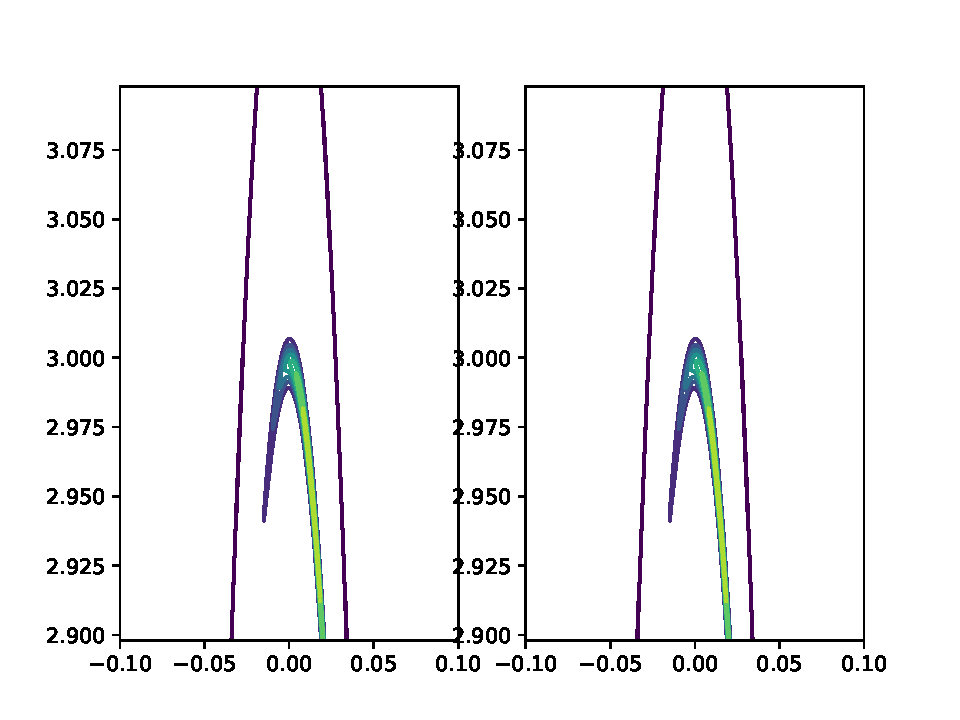
\includegraphics[width=\textwidth]{figures/banana_density}
    \caption{
        Density of the banana model posterior with \(a = 20\), \(b = m = 0\), 
        \(\sigma_1^2 = 20\), \(\sigma_2^2 = 2.5\) and \(\sigma_0^2 = 1000\).
        The blue points are 1000 samples from the posterior.
    }
    \label{banana_density_fig}
\end{figure}

\chapter{Differentially Private MCMC}

As seen in Section~\ref{DP_background}, an algorithm can be made differentially 
private by adding Gaussian noise the its output. The noise could also be added 
to any intermediate value calculated by the algorithm, and post processing immunity 
will guarantee that the same DP bounds that hold for releasing the intermediate 
value also hold for releasing the final result of the algorithm.

In 2019, Yildirim and Ermis~\cite{YildirimE19} realised that if Gaussian noise is added to 
the exact value of \(\lambda\), the noise can be corrected for 
yielding a differentially private MCMC algorithm which converges to 
the correct distribution. In the same year, Heikkilä et.\ al.~\cite{HeikkilaJDH19}
developed another DP MCMC algorithm, called DP Barker, which uses subsampling 
to amplify privacy.

\section{DP Penalty}

In 1999, Ceperley and Dewing~\cite{CeD99} developed a variant of 
Metropolis-Hastings called the penalty 
algorithm, where only a noisy approximation of \(\lambda\) is known. They 
developed the algorithm for simulations in physics where computing \(\lambda\)
requires computing energies of complex systems, which can only be approximated.
The penalty algorithm modifies the acceptance probability to account for the 
noise added to \(\lambda\) and still converges to the correct distribution if 
the noise is Gaussian with known variance.

The DP penalty algorithm adds Gaussian noise to the value of \(\lambda\), and 
uses the penalty algorithm to correct the acceptance probability so that 
the algorithm still converges to the correct distribution~\cite{YildirimE19}.
The corrected acceptance probability for Gaussian noise with variance 
\(\sigma^2\) is 
\[
    \min\{1, e^{\lambda(\theta, \theta') - \frac{1}{2}\sigma^2}\}
\]

Theorem~\ref{DP_penalty_theorem_zcdp} gives the number of iterations DP penalty 
can be run for when the privacy cost is computed through zCDP, which is 
what Yildirim and Ermis prove in their paper~\cite{YildirimE19}. A tighter, but 
harder to use, bound can be reached without using zCDP. This is given by 
Theorem~\ref{DP_penalty_theorem_adp}.

\begin{theorem}\label{DP_penalty_theorem_zcdp}
    Let \(\epsilon > 0\), \(0 < \delta < 1\), \(\alpha > 0\) and \(\tau > 0\).
    Let
    \[
        \rho = (\sqrt{\epsilon - \ln \delta} - \sqrt{-\ln \delta})^2
    \]
    \[
        c(\theta, \theta') = \sup_{x_j, x'_j} (p(x_j\mid \theta') - p(x_j\mid \theta) 
        - (p(x'_j\mid \theta') - p(x'_j\mid \theta)))
    \]
    \[
        \sigma^2(\theta, \theta') = \tau^2 n^{2\alpha}c^2(\theta, \theta')
    \]
    Then DP penalty can be run for 
    \[
        k = \lfloor 2\tau^2 n^{2\alpha} \rho\rfloor
    \]
    iterations when using \(\sigma^2\) as the variance of the Gaussian noise.
\end{theorem}

\begin{theorem}\label{DP_penalty_theorem_adp}
    Let \(\epsilon > 0\) and \(\tau > 0\).
    Define \(c\) and \(\sigma\) as in Theorem~\ref{DP_penalty_theorem_zcdp}.
    The DP penalty algorithm, after running for \(k\) iterations using \(\sigma\)
    as the noise variance, 
    is \((\epsilon, \delta(\epsilon))\)-DP for
    \[
        \delta(\epsilon) 
        = \frac{1}{2}\left(
            \erfc\left(\frac{\epsilon - k\mu}{2\sqrt{k\mu}}\right)
            - e^\epsilon \erfc\left(\frac{\epsilon + k\mu}{2\sqrt{k\mu}}\right)
        \right)
    \]
    where \(\mu = \frac{1}{2\tau^2 n^{2\alpha}}\).
\end{theorem}
\begin{proof}
    DP penalty is an adaptive composition of Gaussian mechanisms that release 
    noisy values of \(\lambda(\theta, \theta')\). The sensitivity of 
    \(\lambda(\theta, \theta')\) is 
    \(c(\theta, \theta')\). For the tight ADP bound used here, the sensitivity must be 
    constant in each iteration. This is achieved by releasing 
    \(\frac{\lambda(\theta, \theta')}{c(\theta, \theta')}\) instead, which 
    has sensitivity 1. \(c(\theta, \theta')\) does not depend on \(X\), 
    so \(\lambda(\theta, \theta')\) can be obtained from 
    \(\frac{\lambda(\theta, \theta')}{c(\theta, \theta')}\) by post processing.

    Adding Gaussian noise with variance \(\sigma_n^2\) to 
    \(\frac{\lambda(\theta, \theta')}{c(\theta, \theta')}\)
    is equivalent to adding Gaussian noise with variance 
    \(\sigma_n^2 c^2(\theta, \theta')\) to \(\lambda(\theta, \theta')\).
    Setting \(\sigma_n^2 = \tau^2n^{2\alpha}\) and plugging into 
    the ADP bound of Theorem~\ref{gauss-DP-bounds} proves the 
    claim.
\end{proof}

Theorem~\ref{DP_penalty_theorem_adp} is harder to use than 
Theorem~\ref{DP_penalty_theorem_zcdp} because the number of iteration 
DP penalty can be run for given an \((\epsilon, \delta)\)-bound cannot be 
computed analytically for the former. However, the maximum number of iterations 
can be solved for numerically.

Theorems~\ref{DP_penalty_theorem_zcdp} and~\ref{DP_penalty_theorem_adp}
require a bound on sensitivity of the log likelihood ratio. If there is a bound 
\[
    |\ln p(x_j\mid \theta') - \ln p(x_j\mid \theta)| \leq L||\theta - \theta'||_2
\]
for all \(D_j, \theta\) and \(\theta'\) then 
\[
    c(\theta, \theta') \leq 2L||\theta - \theta'||_2
\]
The former bound is true in some model, such as logistic regression. In other 
models it can be forced by clipping the log likelihood ratios to the interval 
\([-L||\theta - \theta'||_2, L||\theta - \theta'||_2]\). This will remove the 
guarantee of eventually converging to the correct posterior, but if \(L\) is 
chosen to be large enough, the clipping will not affect the 
acceptance decision frequently. As a tradeoff, picking a large \(L\) will increase 
the variance of the Gaussian noise and slow down convergence through it.

Yildirim and Ermis~\cite{YildirimE19} propose two potential ways to improve the 
performance of the penalty algorithm. The first improvement is only proposing 
changes in one dimension in a multidimensional problem. This decreases 
\(||\theta - \theta'||_2\), which means that it decreases the noise variance.

The second improvement is called \emph{guided random walk} (GRW)~\cite{YildirimE19}.
In GRW, proposals change only one dimension, as above. Additionally, a direction 
is associated with each dimension, and proposals are only made the current 
direction of the chosen dimension. After an accepted proposal, the direction is 
kept the same, but after a reject it is switched. This means that the chain can
move towards areas of higher probability faster because, after some initial 
proposals are rejected, the directions for each dimension point towards the 
area of high probability, so all proposals are towards it. Without GRW, most 
proposals would move the chain away from the area of high probability, and 
would likely be rejected.

\section{DP Barker}

The DP Barker algorithm of Heikkilä et.\ al.~\cite{HeikkilaJDH19} is based on 
the Barker acceptance test~\cite{Barker65} instead of the Metropolis-Hastings test.
Instead of using the MH acceptance probability, the Barker acceptance test samples 
\(V_{log}\sim \mathrm{Logistic(0, 1)}\) and accepts if 
\[
    \lambda + V_{log} > 0
\]

If Gaussian noise with variance \(\sigma^2\) is added to 
\(\lambda\), there exists a correction 
distribution \(V_{corr}\) such that \(\caln(0, \sigma^2) + V_{corr}\) has the 
same distribution as \(V_{log}\). Because the variance of \(V_{log}\) is 
\(\frac{\pi^2}{3}\)~\cite{HeikkilaJDH19}, the variance of \(V_{corr}\) must be 
\(\frac{\pi^2}{3} - \sigma^2\) which means that there is an upper bound
to the noise variance: \(\sigma^2 < \frac{\pi^2}{3}\). Testing whether 
\(\lambda + \caln(0, \sigma^2) + V_{corr} > 0\) is equivalent to testing 
whether \(\lambda + V_{log} > 0\), which means that it is possible to derive 
a DP MCMC algorithm based on the Barker acceptance test if the correction 
distribution can be sampled from.

However, the analytical form of \(V_{corr}\) is not known~\cite{HeikkilaJDH19}.
Heikkilä et.\ al.\  approximate the distribution with a Gaussian mixture model. 
This means that their 
algorithm only converges to an approximately correct distribution, but the 
approximation error can be made very small.

If the sum in \(\lambda\) was only computed over a subset of the data, the 
algorithm would take less computation to run, and would be less sensitive 
to changes in the data. The latter property is called \emph{subsampling amplification}
of differential privacy~\cite{WangBK19}. Using the \(\lambda\) computed 
with subsampling instead of the full data \(\lambda\) introduces an additional 
error that must be corrected for to have the algorithm converge to the correct 
distribution. 

The \emph{central limit theorem} (CLT) states that the distribution of a sum 
of random variables approaches a Gaussian distribution as more random variables 
are summed, if some conditions on the independence and variance of the random 
variables are met~\cite{HeikkilaJDH19}. With the CLT, it can be argued 
that the error from 
using the subsampled \(\lambda\) instead of the full data \(\lambda\) has an 
approximately Gaussian distribution, if the subsample is large 
enough~\cite{HeikkilaJDH19}. 

The variance of the error from subsampling can 
be estimated by the sample variance of the individual terms in the sum in 
\(\lambda\)~\cite{HeikkilaJDH19}. This allows combining the errors from subsampling and the 
Gaussian noise from the Gaussian mechanism to a single Gaussian noise value.
The \(V_{corr}\) distribution can then be used to approximate the Barker acceptance 
test as above. See algorithm~\ref{DP_barker_algo} for the DP Barker algorithm.
\footnote{
    See~\cite{HeikkilaJDH19} for the sampling procedure of \(V_{corr}\).
}

Heikkilä et.\ al.~\cite{HeikkilaJDH19} do not directly bound the sensitivity 
of \(\lambda\) as is done in DP penalty, because the sample variance also 
depends on input data. Instead they directly bound the Rényi divergence 
between \(\caln(0, \sigma^2 - \sigma^2_b)\), where \(\sigma^2_b\) is the 
batch sample variance, for two adjacent inputs. Subsampling amplification 
is accounted for with an amplification theorem for Rényi DP~\cite{WangBK19}.

\begin{theorem}\label{dp_barker_theorem}
    If 
    \[
        |\ln p(x_j\mid \theta') - \ln p(x_j\mid \theta)| \leq \frac{\sqrt{|B|}}{n}
    \]
    \[
        \alpha < \frac{|B|}{5}, \alpha \in \N
    \]
    for all \(\theta, \theta' \in \Theta\), all \(X\) and \(1\leq j \leq n\),
    running \(k\) iterations of DP Barker is \((\alpha, k\epsilon(\alpha))\)-RDP, 
    with 
    \[
        \epsilon(\alpha) = \frac{1}{\alpha - 1}\ln \left(
        1 + q^2\binom{\alpha}{2}\min\{4(e^{\epsilon'(2)} - 1), 2e^{\epsilon'(2)}\}
        + 2 \sum_{j=3}^\alpha q^j\binom{\alpha}{j}e^{(j-1)\epsilon'(j)}\right)
    \]
    and 
    \[
        \epsilon'(\alpha) = \frac{5}{2|B|} + \frac{1}{2(\alpha - 1)}
        \ln \frac{2|B|}{|B| - 5\alpha} + \frac{2\alpha}{|B| - 5\alpha}
    \]
    where \(n\) is the number of rows in \(D\), \(|B|\) is the size of the 
    minibatch and \(q = \frac{|B|}{n}\).
\end{theorem}

Like DP penalty, DP Barker requires a bound on the log likelihood ratio for 
one row of data. The bound can be forced through clipping if the model does not 
meet it, but because of the \(n\) in the denominator of the bound, it can get 
very tight for large values of \(n\). As a result, clipping may be needed for 
almost all log likelihood ratios, which may cause the algorithm to converge 
to a very different distribution from the posterior.

To alleviate the tight bound on log likelihood sensitivity, DP Barker is best 
used with a tempered likelihood~\cite{HeikkilaJDH19}. In tempering, the 
log likelihood is multiplied by a number \(T = \frac{n_0}{n} < 1\). This 
increases the variance of the resulting posterior and may lower modeling 
error in some cases~\cite{HeikkilaJDH19}.

Using the tempered likelihood, the log likelihood 
bound becomes 
\[
    T|\ln p(x_j\mid \theta') - \ln p(x_j\mid \theta)|
    \leq \frac{\sqrt{|B|}}{n}
\]
which is equivalent to 
\[
    |\ln p(x_j\mid \theta') - \ln p(x_j\mid \theta)|
    \leq \frac{\sqrt{|B|}}{n_0}
\]
Typically \(n_0 \ll n\) for large datasets, so using a tempered likelihood requires 
significantly less clipping than a nontempered likelihood.

\begin{algorithm}[H]\label{DP_barker_algo}
    \SetAlgoLined
    \For{\(1 \leq i \leq k\)}{
        denote \(\theta = \theta\)\\
        sample \(\theta' \sim q(\theta)\)\\
        sample \(B \subset \{1, \dotsc, n\}\)\\
        \For{\(j \in B\)}{
            \(r_j = \ln p(\theta'\mid x_j) - \ln p(\theta\mid x_j)\)\\
        }
        \(\sigma^2_b = \mathrm{Var}\{r_j\mid j\in B\}\)\\
        \(\lambda = 
        \frac{n}{|B|}\sum_{j\in B} r_j
        + \ln \frac{p(\theta')}{p(\theta)}
        + \ln \frac{q(\theta\mid \theta')}{q(\theta'\mid \theta)}\)
        \\
        sample \(s \sim \caln(0, \sigma^2 - \sigma^2_b)\)\\
        sample \(c \sim V_{corr}^{\sigma^2}\)\\
        \(\theta_i = \begin{cases}
            \theta' & \text{ if } \lambda + s + c > 0 \\
            \theta & \text{ otherwise}
        \end{cases}
        \)\\
    }
    \Return \((\theta_1, \dotsc, \theta_k)\)
    \caption{
        DP Barker
    }
\end{algorithm}

\section{Comparing DP Penalty and DP Barker}

\chapter{Variations of the Penalty Algorithm}

\section{The Penalty Algorithm with Subsampling}

In the DP Barker algorithm, the log likelihood ratio is computed using only 
a subsample of the dataset to amplify privacy. Subsampling can also be used 
with the penalty algorithm in the same way, if the acceptance test is 
corrected for the subsampling.

As with DP Barker, the error from subsampling is approximately normally 
distributed by the central limit theorem. The variance of the subsampling 
error can be estimated from the sample variance of individual terms of the 
sum in the log likelihood ratio. This means that the penalty method can be used 
to correct for the subsampling error.

The acceptance probability with subsampling is
\[
    \min\{1, e^{\lambda^*(\theta, \theta') - \frac{1}{2}(\sigma^2 + \sigma_b^2)}\},
\]
where
\[
    \lambda^*(\theta, \theta') = \frac{nT}{|B|}\sum_{j\in B}
    \ln \frac{p(x_j\mid \theta')}{p(x_j \mid \theta)}
    + \ln \frac{p(\theta')q(\theta \mid \theta')}{p(\theta)q(\theta' \mid \theta)},
\]
and \(\sigma_b^2\) is the sample variance of the log likelihood ratios in 
batch \(B\). Denote
\[
    r_j = \ln \frac{p(x_j\mid \theta')}{p(x_j\mid \theta)},
\]
\[
    R = \sum_{x\in B}r_j.
\]
Then \(\sigma^2_b\) can be estimated from the sample variance of \(r_j\):
\begin{align*}
    \sigma_b^2 
    &= \var\left(\frac{nT}{|B|}\sum_{j\in B}r_j\right)
    = \frac{nT^2}{|B|^2}\sum_{j\in B}\var(r_j)
    = \frac{nT^2}{|B|}\var(r_j)
  \\&\approx\frac{(nT)^2}{|B|^2}
    \sum_{j\in B}\left(r_j - \frac{R}{|B|}\right)^2
    = \frac{(nT)^2}{|B|^2}\left(\sum_{j\in B}r_j^2 - \frac{R^2}{|B|}\right).
\end{align*}

Because \(\sigma_b^2\) depends on the data, releasing \(\lambda\) privately is 
not enough, \(\lambda - \frac{1}{2}\sigma_b^2\) must be released privately.
This means that using subsampling requires adding additional noise to account 
for the sensitivity of \(\frac{1}{2}\sigma_b^2\).

The sensitivity of \(\lambda - \frac{1}{2}\sigma_b^2\) is 
\[
    \Delta \lambda + \frac{1}{2}\Delta \sigma_b^2.
\]
With the bound \(r_j \leq L||\theta - \theta'||_2\) used in DP penalty, the 
bound sensitivity of \(\lambda\) is the same as without subsampling.
The sensitivity of \(\sigma_b^2\) must be bounded separately.
\begin{lemma}\label{variance_sensitivity_lemma}
    The sensitivity of \(\frac{1}{2}\sigma_b^2\), 
    with \(r_j \leq L||\theta - \theta'||_2\), has upper bound
    \begin{align*}
        \frac{1}{2}\Delta \sigma_b^2
        &\leq \left(\frac{nT}{b}\right)^2 \left|1 - \frac{1}{b}\right|
        L^2||\theta - \theta'||_2^2
        + \frac{2(b - 1)}{b}\left(\frac{nT}{b}\right)^2 L^2||\theta - \theta'||^2_2.
    \end{align*}
\end{lemma}
\begin{proof}
    For datasets \(X \sim X'\), that only differ in one element, denote the 
    common part they have by \(X^*\), and the differing element by \(x\in X\) 
    and \(x'\in X'\)
    \begin{align*}
        \Delta \sigma^2_b &= \sup_{D\sim D'} |\sigma^2_b(X) - \sigma^2_b(X')|
        \\&= \left(\frac{nT}{b}\right)^2 \sup_{X\sim X'}\Big|
        \sum_{x\in X}r^2(x) - \sum_{x\in X'}r^2(x)
        + \frac{1}{b}R^2(X') - \frac{1}{b}R^2(X)\Big|
        \\&= \left(\frac{nT}{b}\right)^2 \sup_{x, x', X^*}\Big|
        r^2(x) - r^2(x')
        + \frac{1}{b}(R(X^*) + r(x'))^2 - \frac{1}{b}(R(X^*) + r(x))^2\Big|
        \\&= \left(\frac{nT}{b}\right)^2 \sup_{x, x', X^*}\Big|
        r^2(x) - r^2(x')
        + \frac{1}{b}(R^2(X^*) + 2R(X^*)r(x') + r^2(x'))
        \\&- \frac{1}{b}(R^2(X^*) + 2R(X^*)r(x) + r^2(x))\Big|
        \\&= \left(\frac{nT}{b}\right)^2 \sup_{x, x', X^*}\Big|
        \left(1 - \frac{1}{b}\right)(r^2(x) - r^2(x'))
        + \frac{2}{b}D(X^*)(r(x') - r(x))\Bigg|
        \\&\leq \left(\frac{nT}{b}\right)^2 \left|1 - \frac{1}{b}\right|
        \sup_{x, x'}\Big|(r^2(x) - r^2(x'))\Big|
        + \frac{2}{b}\left(\frac{nT}{b}\right)^2 \sup_{x, x', X^*}\Big|
        R(X^*)(r(x') - r(x))\Bigg|
        \\&= \left(\frac{nT}{b}\right)^2 \left|1 - \frac{1}{b}\right|
        \sup_{x, x'}\Big|(r^2(x) - r^2(x'))\Big|
        + \frac{2}{b}\left(\frac{nT}{b}\right)^2
        \sup_{x, x'}|r(x') - r(x)|
        \sup_{X^*}|R(X^*)|
        \\&\leq \left(\frac{nT}{b}\right)^2 \left|1 - \frac{1}{b}\right|
        \sup_{x, x'}\Big|(r^2(x) - r^2(x'))\Big|
        + \frac{2}{b}\left(\frac{nT}{b}\right)^2
        \sup_{x, x'}|r(x') - r(x)|(b - 1)\sup_{d}|r(x)|.
    \end{align*}
    Plugging the bound \(\sup_x |r(x)| \leq L||\theta - \theta'||_2\) 
    into the last expression proves the claim.
\end{proof}

\begin{theorem}
    Let
    \[
        \Delta_\lambda = \frac{2nTL}{|B|}||\theta - \theta'||_2,
    \]
    \[
        \Delta_\sigma = \left(\frac{nT}{b}\right)^2 \left|1 - \frac{1}{b}\right|
        L^2||\theta - \theta'||_2^2,
        + \frac{2(b - 1)}{b}\left(\frac{nT}{b}\right)^2 L^2||\theta - \theta'||^2_2.
    \]
    \[
        c(\theta, \theta') = \Delta_\lambda + \Delta_\sigma,
    \]
    \[
        \sigma^2(\theta, \theta') = \tau c^2(\theta, \theta').
    \]
    Then running DP penalty with subsampling for \(k\) iterations 
    is \((\alpha, k\epsilon(\alpha))\)-RDP, with
    \[
        \epsilon(\alpha) = \frac{1}{\alpha - 1}\ln \left(
        1 + q^2\binom{\alpha}{2}\min\{4(e^{\epsilon'(2)} - 1), 2e^{\epsilon'(2)}\}
        + 2 \sum_{j=3}^\alpha q^j\binom{\alpha}{j}e^{(j-1)\epsilon'(j)}\right),
    \]
    and 
    \[
        \epsilon'(\alpha) = \frac{\alpha}{2\tau},
    \]
    where \(n\) is the number of rows in \(D\), \(|B|\) is the size of the 
    minibatch and \(q = \frac{|B|}{n}\).
\end{theorem}
\begin{proof}
    By Lemma~\ref{variance_sensitivity_lemma}, 
    \(\Delta_\sigma(\theta, \theta')\) an upper 
    bound to the sensitivity of \(\frac{1}{2}\sigma_b^2\), therefore 
    \(c(\theta, \theta')\) is an upper bound to the sensitivity of 
    \(\lambda - \frac{1}{2}\sigma_b^2\).

    This means that a Gaussian mechanism taking a subsample \(B\) of the data as 
    input and uses \(\sigma(\theta, \theta')\) as the noise variance 
    is \((\alpha, \epsilon'(\alpha))\)-RDP with 
    \[
        \epsilon'(\alpha) = \frac{\alpha}{2\tau}.
    \]
    By the subsampling amplification theorem~\cite[Theorem 9]{WangBK19} and 
    the composition theorem of RDP (Theorem~\ref{composition-theorem}),
    the combination of subsampling and Gaussian mechanism is 
    \((\alpha, k\epsilon(\alpha))\)-RDP with 
    \[
        \epsilon(\alpha) = \frac{1}{\alpha - 1}\ln \left(
        1 + q^2\binom{\alpha}{2}\min\{4(e^{\epsilon'(2)} - 1), 2e^{\epsilon'(2)}\}
        + 2 \sum_{j=3}^\alpha q^j\binom{\alpha}{j}e^{(j-1)\epsilon'(j)}\right)
    \]
    when run for \(k\) iterations for integer \(\alpha \geq 2\).
\end{proof}

The appearance of \(n\) as a multiplier of \(\Delta_\lambda\) and 
\(n^2\) as a multiplier of \(\Delta_\sigma\) causes the noise variance to increase 
with \(n\), without a corresponding decrease in \(\epsilon'\). This makes subsampled 
DP penalty unsuitable for problems with large datasets, unless tempering is 
used. Like with DP Barker, using tempering \(T = \frac{n_0}{n}\) cancels \(n\)
out of the noise variance.

% \section{DP Metropolis-Adjusted Langevin Algorithm}
%
% Metropolis adjusted Langevin algorithm (MALA)~\cite{Roberts1998} 
% is Metropolis-Hastings with the proposal distribution 
% \[
%     q(\theta' \mid \theta, X) = \caln\left(\theta + \frac{1}{2}\sigma^2_p
%     \nabla \ln p(X\mid \theta), \sigma^2_p I\right)
% \]
% The gradient in the proposal is meant to guide the random walk to regions 
% of high probability. Because of it, MALA can achieve a higher acceptance rate 
% than standards random walk MH, and requires fewer iterations to 
% converge~\cite{Roberts1998}.
%
% MALA can be made DP with using the penalty algorithm. Because MALA is just 
% the MH algorithm with a particular proposal, the penalty algorithm using the 
% MALA proposal will converge to the correct distribution. Proving any DP bound 
% for MALA requires computing the sensitivities of the different data-dependent 
% values that the algorithm computes.
%
% Like random walk MH, the acceptance probability for non-DP MALA is
% \[
%     p = \min\left\{1, \exp(\lambda(X, \theta, \theta'))\right\},
% \]
% with 
% \[
%     \lambda(X, \theta, \theta') 
%     = \sum_{x\in X} \ln\frac{p(x\mid \theta')}{p(x\mid \theta)} 
%     + \ln \frac{q(\theta\mid \theta', X)} {q(\theta'\mid \theta, X)}
%     + \ln \frac{p(\theta')}{p(\theta)}.
% \]
%
% For DP MALA, the penalty correction is applied, and the acceptance probability is
% \[
%     p = \min\left\{\exp\left(\lambda^*(X, \theta, \theta')
%     - \frac{1}{2}\sigma^2(\theta, \theta')\right)\right\}
% \]
% where \(\lambda^*(X, \theta, \theta') \sim \caln(\lambda(X, \theta, \theta'), 
% \sigma^2(\theta, \theta'))\) and \(\sigma^2\) is symmetric in \(\theta\) and 
% \(\theta'\).
%
% \begin{algorithm}[H]
%     \SetAlgoLined 
%     \For{\(1 \leq i \leq k\)}{
%         sample \(\theta'\) from 
%         \(\calm_g(\theta_{i-1} + \frac{1}{2}\sigma_p^2\nabla \ln p(X\mid \theta_{i-1}))\)\\
%         sample \(\lambda^*\) from \(\calm_l(\lambda)\)\\
%         \(p = \min\left\{1, \exp\left(\lambda^* - \frac{1}{2}\sigma^2\right)\right\}\)\\
%         \(\theta_i = \begin{cases}
%             \theta^* & \text{ with probability } p \\
%             \theta_{i-1} & \text{ otherwise }
%         \end{cases}\)
%     }
%     \caption{DP MALA
%     }
% \end{algorithm}
%
% On each iteration, the proposal \(\theta'\) is sampled from a Gaussian 
% mechanism \(\calm_g(\theta + \frac{1}{2}\sigma^2_p\nabla \ln p(X\mid \theta))\)
% with variance \(a\sigma_p^2\).
% Then \(\lambda^*(X, \theta, \theta')\) is sampled from a 
% Gaussian mechanism \(\calm_l(\lambda(X, \theta, \theta'))\) with variance 
% \(\sigma^2\). The reason for using variance \(a\sigma^2_p\) for the proposal 
% instead of \(\sigma^2_p\) that non-DP MALA uses is to allow better adjustment 
% of the privacy cost of the proposal.
%
% \begin{lemma}\label{dp_mala_gradient}
%     \(\calm_g\) is \(\rho_g\)-zCDP with 
%     \[
%         \rho_g(\theta) = \frac{\sigma_p^2 c_g^2}{8a}
%     \]
%     where 
%     \[
%         c_g \geq \Delta_2 \nabla \ln p(X\mid \theta)
%     \]
% \end{lemma}
% \begin{proof}
%     The sensitivity of 
%     \[
%         \frac{1}{2}\sigma_p^2 \nabla \ln p(X\mid \theta)
%     \]
%     is 
%     \[
%         \frac{1}{2}\sigma_p^2 \nabla \Delta_2 \nabla \ln p(X\mid \theta)
%     \]
%     The zCDP bound follows from Theorem~\ref{gauss-DP-bounds}.
% \end{proof}
%
% \(c_g\) cannot depend on \(\theta\) as the privacy cost of each iteration in 
% a composition must be determinable ahead of time to apply 
% Theorem~\ref{composition-theorem}.
%
% \begin{lemma}\label{dp_mala_likelihood_bound}
%     \(\calm_l\) is \(\rho_l\)-zCDP with 
%     \[
%         \rho_l = \frac{1}{2\tau},
%     \]
%     when 
%     \[
%         c_l(\theta, \theta') = \Delta_2^2 \lambda(X, \theta, \theta'),
%     \]
%     and
%     \[
%         \sigma^2(\theta, \theta') = \tau c^2_l(\theta, \theta').
%     \]
% \end{lemma}
% \begin{proof}
%     By Theorem~\ref{gauss-DP-bounds}, \(\calm_l\) is \(\rho\)-zCDP with
%     \[
%         \rho_l = \frac{c_l^2(\theta, \theta')}{2\sigma^2(\theta, \theta')}.
%     \]
%     The claim follows from plugging in \(\sigma(\theta, \theta')\).
% \end{proof}
%
% \begin{theorem}\label{dp_mala_zcdp_bound}
%     With given ADP bounds \(\epsilon\) and \(\delta\),
%     DP MALA can be run for 
%     \[
%         k = \left\lfloor \frac{\rho}{\rho_g + \rho_l} \right\rfloor
%     \]
%     iterations, where \(\rho_g\) is from Lemma~\ref{dp_mala_gradient},
%     \(\rho_l\) is from Lemma~\ref{dp_mala_likelihood_bound}, and
%     \[
%         \rho = \left(\sqrt{\log \frac{1}{\delta} + \epsilon} 
%         - \sqrt{\log \frac{1}{\delta}}\right)^2
%     \]
% \end{theorem}
% \begin{proof}
%     A single iteration is \((\rho_l + \rho_g)\)-zCDP. The claim then follows from 
%     Theorems~\ref{other_dp_to_adp} and~\ref{composition-theorem}.
% \end{proof}
%
% The zCDP bounds of DP MALA can be computed with Theorem~\ref{dp_mala_zcdp_bound}
% if the sensitivities \(c_g\) and \(c_l\) are known. As in DP penalty, they are 
% specific the likelihood, but they can be forced with clipping. Clipping the 
% gradients does not affect the distribution the algorithm converges to, but can 
% diminish the amount of utility the algorithm can get from the gradients.
% Clipping the likelihood does change the invariant distribution, but if the clipping 
% is limited the algorithm should remain accurate.
%
% Clipping the gradients of each individual iteration results in
% \begin{align*}
%     ||\nabla \log p(X\mid \theta) - \nabla \log p(X'\mid \theta)||_2
%     &= ||\nabla \log p(x\mid \theta) - \nabla \log p(x'\mid \theta)||_2
%     \leq 2L_g
% \end{align*}
% so 
% \[
%     c_g(\theta) = 2L_g
% \]
% and 
% \[
%     \rho_g = \frac{\sigma_p^2L_g^2}{2a}.
% \]
%
% \(c_l\) consists of two term that depend on the data, the 
% log likelihood term 
% \[
%     \sum_{i=1}^n \ln \frac{p(x_i\mid \theta')}{p(x_i\mid \theta)}
% \]
% and the log proposal ratio
% \[
%     \ln \frac{q(\theta\mid \theta', X)}{q(\theta'\mid \theta, X)}
% \]
%
% The log likelihood term is the same that appears in DP penalty, and can be 
% bound in the same way. If it is clipped such that
% \(\left|\log \frac{p(x\mid \theta')}{p(x\mid \theta)}\right| \leq L||\theta - \theta'||_2\)
% then
% \[
%     \Delta\left(\sum_{x_in X}\log \frac{p(x\mid \theta')}{p(x\mid \theta)}\right)
%     \leq 2L||\theta - \theta'||_2.
% \]
%
% The log proposal term does not appear in DP penalty, because it uses a symmetric 
% proposal where the term is always 0. In DP MALA, the proposal is not symmetric, 
% and depends on the data through \(\nabla \ln p(X\mid \theta)\), so the term 
% must be included in the sensitivity calculation.
%
% Let \(d\) be the dimensionality of \(\theta\). Then
% \[
%     q(\theta\mid \theta', X) = \prod_{i=1}^d
%     \frac{1}{\sqrt{2\pi a\sigma_p^2}}\exp\left(
%     \frac{(\theta_i - \theta_i' - \frac{1}{2}\sigma_p^2
%     \frac{\partial}{\partial \theta'_i} \log p(X, \theta'))^2}
%     {2a\sigma_p^2}\right)
% \]
% \begin{align*}
%     \log \frac{q(\theta\mid \theta', X)}{q(\theta'\mid \theta, X)}
%     &= \sum_{i=1}^d \left(C +
%     \frac{(\theta_i - \theta'_i
%     - \frac{1}{2}\sigma_p^2\frac{\partial}{\partial \theta_i'} \log p(X\mid \theta'))^2}
%     {2a\sigma_p^2}\right)
%     - \sum_{i=1}^d \left(C +
%     \frac{(\theta_i' - \theta_i 
%     - \frac{1}{2}\sigma_p^2\frac{\partial}{\partial \theta_i} \log p(X\mid \theta))^2}
%     {2a\sigma_p^2}\right)
%   \\&=\frac{1}{2a\sigma_p^2} \sum_{i=1}^d \left(
%     (\theta_i - \theta'_i
%     - \frac{1}{2}\sigma_p^2\frac{\partial}{\partial \theta_i'} \log p(X\mid \theta'))^2
%     - (\theta_i' - \theta_i 
%     - \frac{1}{2}\sigma_p^2\frac{\partial}{\partial \theta_i} \log p(X\mid \theta))^2
%     \right)
%   \\&=\frac{1}{2a\sigma_p^2} \sum_{i=1}^d \left(
%     (\theta_i - \theta'_i - G_i(X\mid \theta'))^2
%     - (\theta_i' - \theta_i - G_i(X\mid \theta))^2\right)
% \end{align*}
%
% Let 
% \[
%     G_i(X\mid \theta) = \frac{1}{2}\sigma_p^2\frac{\partial}{\partial \theta_i}
%     \log p(X\mid \theta)
% \]
% As 
% \[
%     \log p(X\mid \theta) = \sum_{x\in X}\log p(x\mid \theta)
% \]
% if \(X\) and \(X'\) only differ in one row, those being \(x\) and \(x'\),
% then
% \begin{align*}
%     G_i(X\mid \theta) - G_i(X'\mid \theta) 
%     &= \frac{1}{2}\sigma_p^2\sum_{j=1}^n \frac{\partial}{\partial \theta_i}
%     (\log p(x_j\mid \theta) - \log p(x'_j\mid \theta))
%   \\&= \frac{1}{2}\sigma_p^2 \frac{\partial}{\partial \theta_i}
%     (\log p(x\mid \theta) - \log p(x'\mid \theta))
%   \\&= G_i(x\mid \theta) - G_i(x'\mid \theta)
% \end{align*}
% Let \(X^*\) be the equal part of \(X\) and \(X'\). Then 
% \[
% G_i(X\mid \theta) = G_i(X^*\mid \theta) + G_i(x\mid \theta)
% \]
% and 
% \[
%     G_i(X'\mid \theta) = G_i(X^*\mid \theta) + G_i(x'\mid \theta)
% \]
%
% Additionally
% \[
%     (a + b)^2 - (a + c)^2 = 2a(b - c) + b^2 - c^2
% \]
% for any \(a, b, c\in \R\).
%
% Let 
% \[
% \Delta(X) = \left|\log \frac{q(\theta\mid \theta',X)}{q(\theta'\mid \theta,X)} 
% - \log \frac{q(\theta\mid \theta',X)}{q(\theta'\mid \theta,X)}\right|
% \]
% \begin{align*}
%     \Delta(X) 
%     &=
%     \frac{1}{2a\sigma_p^2}
%     \Bigg|\sum_{i=1}^d (\theta_i - \theta'_i - G_i(X\mid \theta'))^2
%     - (\theta'_i - \theta_i - G_i(X\mid \theta))^2
%   \\&- (\theta_i - \theta'_i - G_i(X'\mid \theta'))^2
%     + (\theta'_i - \theta_i - G_i(X'\mid \theta))^2\Bigg|
%   \\&=
%     \frac{1}{2a\sigma_p^2}
%     \Bigg|\sum_{i=1}^d \Big(
%     (\theta_i - \theta'_i)^2 - 2(\theta_i - \theta'_i)G_i(X\mid \theta')
%     + G_i(X\mid \theta')^2
%   \\&- (\theta'_i - \theta_i)^2 + 2(\theta'_i - \theta_i)G_i(X\mid \theta)
%     - G_i(X\mid \theta)^2
%   \\&- (\theta_i - \theta_i')^2 + 2(\theta_i - \theta'_i)G_i(X'\mid \theta')
%     - G_i(X'\mid \theta')^2
%   \\&+ (\theta'_i - \theta_i)^2 - 2(\theta'_i - \theta_i)G_i(X'\mid \theta)
%     + G_i(X'\mid \theta)^2\Big)\Bigg|
%   \\&=
%     \frac{1}{2a\sigma_p^2}
%     \Bigg|\sum_{i=1}^d \Big(
%     2(\theta'_i - \theta_i)(G_i(X\mid \theta) - G_i(X'\mid \theta))
%     + 2(\theta_i - \theta'_i)(G_i(X'\mid \theta') - G_i(X\mid \theta'))
%   \\&+ G_i(X\mid \theta')^2
%     - G_i(X\mid \theta)^2
%     - G_i(X'\mid \theta')^2
%     + G_i(X'\mid \theta)^2\Big)\Bigg|
%   \\&=
%     \frac{1}{2a\sigma_p^2}
%     \Bigg|\sum_{i=1}^d \Big(
%     2(\theta'_i - \theta_i)(G_i(x\mid \theta) - G_i(x'\mid \theta) 
%     + G_i(x\mid \theta') - G_i(x'\mid \theta'))
%   \\&+(G_i(X^*\mid \theta') + G_i(x\mid \theta'))^2
%     - (G_i(X^*\mid \theta') + G_i(x'\mid \theta'))^2
%   \\&+ (G_i(X^*\mid \theta) + G_i(x'\mid \theta))^2
%     - (G_i(X^*\mid \theta) + G_i(x\mid \theta))^2\Big)\Bigg|
%   \\&=
%     \frac{1}{2a\sigma_p^2}
%     \Bigg|\sum_{i=1}^d \Big(
%     2(\theta'_i - \theta_i)(G_i(x\mid \theta) - G_i(x'\mid \theta) 
%     + G_i(x\mid \theta') - G_i(x'\mid \theta'))
%   \\&+ 2G_i(X^*\mid \theta')(G_i(x\mid \theta') - G_i(x'\mid \theta'))
%   + G_i(x\mid \theta')^2 - G_i(x'\mid \theta')^2
%   \\&+ 2G_i(X^*\mid \theta)(G_i(x'\mid \theta) - G_i(x\mid \theta))
%   + G_i(x'\mid \theta)^2 - G_i(x\mid \theta)^2\Big)\Bigg|
%   \\&\leq \frac{1}{2a\sigma_p^2}\Bigg(
%   2\left|(\theta' - \theta)^T(G(x\mid \theta) - G(x'\mid \theta) 
%   + G(x\mid \theta') - G(x'\mid \theta'))\right|
%   \\&+ 2\left|G(X^*\mid \theta')^T(G(x\mid \theta') - G(x'\mid \theta'))\right|
%   + 2\left|G(X^*\mid \theta)^T(G(x'\mid \theta) - G(x\mid \theta))\right|
%   \\&+ |||G(x\mid \theta')||_2^2 - ||G(x'\mid \theta')||_2^2
%   + ||G(x'\mid \theta)||_2^2 - ||G(x\mid \theta)||_2^2|
%   \Bigg)
% \end{align*}
% Continued:
% \begin{align*}
%     \Delta(X)
%     &\leq \frac{1}{2a}
%   \left|(\theta' - \theta)^T(\nabla\log p(x\mid \theta) - \nabla \log p(x'\mid \theta) 
%   + \nabla\log p(x\mid \theta') - \nabla\log p(x'\mid \theta'))\right|
%   \\&+ \frac{\sigma_p^2}{4a}\left|\nabla \log p(X^*\mid \theta')^T(\nabla \log p(x\mid \theta') 
%   - \nabla \log p(x'\mid \theta'))\right|
%   \\&+ \frac{\sigma_p^2}{4a}\left|\nabla \log p(X^*\mid \theta)^T(\nabla \log p(x'\mid \theta) 
%   - \nabla \log p(x\mid \theta))\right|
%   \\&+ \frac{\sigma_p^2}{8a}\Big| ||\nabla \log p(x\mid \theta')||_2^2 
%   - ||\nabla \log p(x'\mid \theta')||_2^2
%   + ||\nabla \log p(x'\mid \theta)||_2^2 
%   - ||\nabla \log p(x\mid \theta)||_2^2\Big|
%   \\&\leq \frac{1}{2a}
%   ||\theta' - \theta||_2||\nabla\log p(x\mid \theta) - \nabla \log p(x'\mid \theta) 
%   + \nabla\log p(x\mid \theta') - \nabla\log p(x'\mid \theta')||_2
%   \\&+ \frac{\sigma_p^2}{4a}||\nabla \log p(X^*\mid \theta')||_2||\nabla \log p(x\mid \theta') 
%   - \nabla \log p(x'\mid \theta')||_2
%   \\&+ \frac{\sigma_p^2}{4a}||\nabla \log p(X^*\mid \theta)||_2||\nabla \log p(x'\mid \theta) 
%   - \nabla \log p(x\mid \theta)||_2
%   \\&+ \frac{\sigma_p^2}{8a}\Big| ||\nabla \log p(x\mid \theta')||_2^2 
%   - ||\nabla \log p(x'\mid \theta')||_2^2
%   + ||\nabla \log p(x'\mid \theta)||_2^2 
%   - ||\nabla \log p(x\mid \theta)||_2^2\Big|
%   \\&\leq \frac{2}{a}L_g||\theta' - \theta||_2 + \frac{\sigma_p^2}{a}(n-1)L_g^2
%   + \frac{\sigma_p^2L_g^2}{2a}
% \end{align*}
% with bound \(||\nabla \log p(x\mid \theta)||_2 \leq L_g\).
% There may be possibility for improving the bound with additional information on
% \(\nabla \log p(x\mid \theta) - \nabla \log p(x\mid \theta')\).
%
% Together with the bound on the log likelihood ration this implies that 
% \[
%     \Delta \lambda(X, \theta, \theta') 
%     \leq 2L||\theta - \theta'||_2 + \frac{2}{a}L_g||\theta - \theta'||_2 
%     + \frac{\sigma_p^2}{a}(n - 1)L_g^2 + \frac{1}{2a}\sigma_p^2L_g^2 
% \]
%
% If there is an additional bound \(||\log p(X\mid \theta)||_2 \leq L_S\), then
% \(||\log p(X^*\mid \theta)||_2 \leq L_S + L_g\) and 
% \[
%     \Delta \lambda(X, \theta, \theta')
%     \leq 2L||\theta - \theta'||_2 + \frac{2}{a}L_g||\theta - \theta'||_2 
%     + \frac{\sigma_p^2}{a}(L_S + L_g) L_g + \frac{1}{2a}\sigma_p^2L_g^2 
% \]
% With large \(n\) this results in a much tighter sensitivity bound than the 
% previous bound.

\chapter{Differentially Private Hamiltonian Monte Carlo}

Hamiltonian Monte Carlo (HMC\footnote{
    HMC originally stood for hybrid Monte Carlo, 
    but the name Hamiltonian Monte Carlo has become more common.
})~\cite{neal2012mcmc} is a widely used MCMC algorithm that, like 
Metropolis-Hastings and the penalty algorithm, was originally developed 
for simulations in physics and chemistry, but has since been applied to 
Bayesian inference. 

HMC simulates the trajectory of a moving particle in a way 
that allows it to draw samples from a target distribution~\cite{neal2012mcmc}. 
With perfect simulation 
an acceptance test would not be needed, but exact simulation of the moving particle 
is typically not possible so a Metropolis-Hastings acceptance test is used
for proposal generated by the simulation. Despite imperfections, the simulation can generate long jumps 
that stay in areas of high probability, giving HMC a higher acceptance rate 
that Metropolis-Hastings using a Gaussian distribution as the proposal, at the 
cost of higher computational requirements.

This chapter first introduces HMC in the non-DP setting in Section~\ref{hmc_basics_section}.
In Section~\ref{dp_hmc_section} the HMC is made differentially private using the 
acceptance test of the penalty algorithm and adding noise to the proposal phase 
appropriately.

\section{MCMC with Hamiltonian Dynamics}\label{hmc_basics_section}

The motion of a particle on a frictionless surface of varying height is governed 
by the initial position and velocity of the particle, and the height of the 
surface at different positions~\cite{neal2012mcmc}. 
The kinetic energy of the particle with 
momentum\footnote{Momentum is velocity times mass.}
\(p \in \R^{2}\) and mass \(m \in \R\) is \(\frac{p^{T}p}{2m}\). The potential energy of the particle
at position \(\theta \in \R^{2}\) is proportional to the height of the surface, given by
a continuously differentiable function \(U(\theta)\). 
The sum of potential and kinetic energies, the total 
energy of the system, is called the Hamiltonian \(H\). Hamilton's equations 
give the equations of motion for a system with a given Hamiltonian:
\begin{align*}
    &\frac{d\theta}{dt} = \frac{\partial H}{\partial p},
    &\frac{dp}{dt} = -\frac{\partial H}{\partial \theta}.
\end{align*}
Given \(H(\theta, p) = U(\theta) + \frac{p^{T}p}{2m}\), Hamilton's equations become
\begin{align*}
    \frac{d\theta}{dt} &= \frac{p}{m}, \\
    \frac{dp}{dt} &= -\nabla U(\theta).
\end{align*}

These equations define a function \(T_t\) taking an initial state 
\((\theta, p)\) of the particle to the state \(T(\theta, p)\) after time \(t\).
Solving \(T_t\) analytically is usually not possible, but \(T_t\) can be 
approximately simulated by the leapfrog method. The leapfrog method sequentially 
updates an estimate \((\theta_i, p_i)\) of the state in steps \(L\) of \(\eta\) 
as follows:
\begin{align*}
    p_{i+1/2} &= p_i - \frac{\eta}{2}\nabla U(\theta_i) \\
    \theta_{i+1} &= \theta_i + \frac{\eta p_{i+1/2}}{m} \\
    p_{i+1} &= p_{i+1/2} - \frac{\eta}{2}\nabla U(\theta_{i+1}) \\
\end{align*}
The simulation starts with \(\theta_0 = \theta\) and \(p_0 = p\) and the 
result is given by \(T_{L\eta}(\theta, p) \approx (\theta_L, p_L)\).

The above equations for two-dimensional \(\theta\) and \(p\) generalize to
any number of dimensions \(d\)~\cite{neal2012mcmc}. The physical analogue would be a particle moving
on a \(d\)-dimensional hypersurface with ``height'' given by \(U(\theta)\).
The mass of the particle, \(m\), can also be generalized to any positive
definite matrix \(M \in \R^{p\times p}\), which changes division by
\(m\) to multiplication by \(M^{-1}\). Specifically, the kinetic energy of the
particle becomes \(\frac{1}{2}p^{T}M^{-1}p\) and
\(\frac{d\theta}{dt} = M^{-1}p\). The generalization to a mass matrix does not
have a physical analogue, but it can be useful for MCMC.

Hamiltonian dynamics have three important properties~\cite{neal2012mcmc} 
that make them useful as a
proposal mechanism for MCMC. They are reversibility, 
conservation of the Hamiltonian and conservation of volume.

Reversibility means that the function \(T_t\) is injective, meaning that
it has an inverse \(T_{-t}\) where \(T_t(\theta_1, p_1) = (\theta_2, p_2)\)
implies that \(T_{-t}(\theta_2, p_2) = (\theta_1, p_1)\)~\cite{neal2012mcmc}.
For the Hamiltonian of the particle moving on a surface, the inverse 
is obtained by \(T_t(\theta_2, -p_2) = (\theta_1, -p_1)\).

Conservation of the Hamiltonian follows from Hamilton's equations and the 
chain rule of derivatives:
\[
    \frac{dH}{dt} = \frac{\partial H}{\partial \theta}\frac{d \theta}{dt}
    + \frac{\partial H}{\partial p}\frac{dp}{dt}
    = \frac{\partial H}{\partial \theta}\frac{\partial H}{\partial p}
    - \frac{\partial H}{\partial p}\frac{\partial H}{\partial \theta}
    = 0.
\]

Conservation of volume in the \((\theta, p)\)-space follows from the fact that 
the absolute value of the Jacobian determinant of \(T_t\) is 1 and the 
injectivity of \(T_t\). A somewhat 
lengthier proof for the Jacobian determinant of \(T_t\) is given by 
Neal~\cite{neal2012mcmc}. 

To see why 
having \(|\det J_f| = 1\), where \(J_f\) is the Jacobian matrix of an injective 
continuously differentiable function \(f\), 
implies \(f\) preserving volume, recall that the volume of a set 
\(A\) is given by 
\[
    \int_A 1dx.
\]
The volume of the image of \(A\) under \(f\), \(f(A)\), is given by
\[
    \int_{f(A)}1dx = \int_{A}|\det J_f(x)|dx = \int_A 1dx.
\]
where the first equality follows from the change of variables formula.

The leapfrog method does not conserve the Hamiltonian exactly, but it 
preserves volumes and is reversible exactly~\cite{neal2012mcmc}. 
These properties of the leapfrog 
method are important for its use as a proposal mechanism for MCMC.

The HMC algorithm samples from the distribution of~\cite{neal2012mcmc}
\[
    P(\theta, p) \propto \exp(-H(\theta, p)).
\]
With \(H(\theta, p) = U(\theta) + \frac{1}{2}p^{T}M^{-1}p\),
\[
    P(\theta, p) \propto \exp(-U(\theta))\exp\left(\frac{1}{2}p^{T}M^{-1}p\right)
\]
This means that the marginal distributions of \(\theta\) and \(p\) are 
independent, the marginal distribution of \(p\) is a d-dimensional
Gaussian distribution 
with mean 0 and covariance \(M\), and the marginal distribution of
\(\theta\) can have any continuously differentiable log likelihood \(-U\).
Because of this, \(\theta\) is used to represent the variables of interest,
while \(p\) is a set of auxiliary variables used for the proposals.

Generating a \((\theta, p)\)-sample is done in two stages~\cite{neal2012mcmc}, 
which are technically 
two separate Metropolis-Hastings proposals and acceptance tests. In the first 
stage, \(p\) is proposed from the Gaussian distribution with mean 0 and 
covariance \(M\). Because the proposal matches the marginal distribution of 
\(p\), it is always accepted.

In the second stage, Hamiltonian dynamics for the particle on a surface are 
simulated with the leapfrog method, starting from the current value 
of \(\theta\) and the proposed value of \(p\). The end result is a proposal 
for both \(\theta\) and \(p\). Because the leapfrog simulation preserves volumes 
and is reversible by negating \(p\), the acceptance probability of the 
proposal is simply
\[
    \min\{1, \exp(H(\theta, p) - H(\theta', p'))\}.
\]
If the simulation conserved \(H\) exactly, the acceptance probability would 
always be 1. Because this is usually not possible, there is always some probability 
of rejecting, which depends on the length of the jump taken by the leapfrog 
method, \(\eta\), and the number of leapfrog steps, \(L\). It might be expected 
that the errors from the leapfrog steps would accumulate during the simulation, 
but in practice the errors in different steps tend to cancel each 
other~\cite{neal2012mcmc}, meaning 
that the acceptance probability mainly depends on \(\eta\).

\section{Differential Privacy with HMC}\label{dp_hmc_section}

HMC only uses the model log likelihood, and thus the data, through \(U\).
\(U\) is used in two ways. Firstly, its value is used in the acceptance test,
and secondly, its gradients are used in to obtain proposals. Adding appropriate
amounts of noise to both accesses would make HMC private, but the addition of
noise may break some of the properties required for the algorithm's correctness.

The addition of noise to the log likelihood ratios can be corrected using the penalty
acceptance test, i.e. changing the acceptance probability to
\[
    \min\left\{\exp\left(H(\theta, p) - H(\theta', p') - \frac{1}{2}\sigma_{l}^{2}\right)\right\},
\]
where \(\sigma_{l}^{2}\) is the variance of the noise added to the log likelihood
ratios. This is because with \(U(\theta) = -\ln p(X\mid \theta)\), the difference
of the Hamiltonians in the acceptance probability is
\[
  H(\theta, p) - H(\theta', p') = \ln p(X\mid \theta') - \ln p(X\mid \theta)
  + \frac{1}{2}(p^{T}M^{-1}p - p'^{T}M^{-1}p').
\]
As with the penalty algorithm, the sensitivity of the log likelihood ratios must
be bounded. If a bound does not exist, clipping must be used, nullifies the asymptotic
converge guarantee of the algorithm. However, in Section~\ref{clipping_experiments}
it is shown that
clipping low numbers of gradients does not affect convergence in practice.

Releasing the gradients privately requires a trade-off. The leapfrog method remains
reversible with noisy and potentially clipped gradients, as is shows in the following,
but they no longer simulate the correct Hamiltonian dynamics~\cite{CFG14}. This does not affect
asymptotic convergence, but it can potentially lower acceptance rates.
The dynamics can be corrected by adding a friction term to the equations of
motion of the simulation~\cite{CFG14}, but this removes volume preservation of the simulation,
which means that the acceptance probability must be corrected.

The leapfrog update equations with noisy and clipped gradients become
\begin{align*}
  p_{i+1/2} &= p_{i} - \frac{\eta}{2}(\clip(\nabla U(\theta_{i})) + \caln(0, \sigma_{g}^{2})) \\
  \theta_{i+1} &= \theta_{i} + \eta M^{-1}p_{i+1/2} \\
  p_{i+1} &= p_{i+1/2} - \frac{\eta}{2}(\clip(\nabla U(\theta_{i+1})) + \caln(0, \sigma_{g}^{2})).
\end{align*}
The second equation is unchanged, and remains both volume preserving and reversible
by negating \(p\). Both the first and third equations apply the function
\(l_{p}\colon \R^{2d}\to \R^{2d}\),
\[
  l_{p}(\theta, p) = \left(\theta, p - \frac{\eta}{2}(\clip(\nabla U(\theta))
    + \caln(0, \sigma_{g^{2}}))\right).
\]
to \(\theta\) and \(p\).

The Jacobian of \(l_{p}\) is
\[
  J_{l_{p}}(\theta, p) =
  \begin{pmatrix}
    I_{d\times d} & 0_{d\times d} \\
    C(\theta, p) & I_{d\times d}
  \end{pmatrix},
\]
where \(I_{d\times d}\) and \(0_{d\times d}\) are the \(d\)-by-\(d\) identity and
zero matrices, respectively, and \(C(\theta, p) = J_{\clip(\nabla U(\theta))}(\theta, p)\).
Because \(J_{l_{p}}(\theta, p)\) is triangular, \(\det J_{l_{p}}(\theta, p) = 1\)
for all \(\theta\) and \(p\), which means that \(l_{p}\) preserves volume.
As the step updating \(\theta\) also preserves volume, the entire leapfrog
simulation preserves volume.

Showing that the leapfrog simulation is reversible by negating \(p\) requires
more thought, as the simulation is no longer deterministic. Recall that the
MH acceptance test uses the acceptance probability
\[
  \min\left\{1, \frac{\pi(\theta')}{\pi(\theta)}
    \frac{q(\theta\mid \theta')}{q(\theta'\mid \theta)}\right\},
\]
where \(\pi\) is the target density and \(q\) is the proposal density.
For HMC, \(q\) must be understood as a Dirac \(\delta\) function, as the
standard leapfrog is deterministic. The reversibility of the leapfrog
by negating \(p\) means that
\(q(\theta', p'\mid \theta, p) = q(\theta, -p\mid \theta', -p')\).
If \(p\) were negated after the leapfrog simulation, one would have another
proposal distribution \(q'\), with
\(q'(\theta', p'\mid \theta, p) = q'(\theta, p\mid \theta', p')\).
Running HMC with proposal \(q'\) instead of \(q\) does not change the
output of the algorithm, as \(p\) is not stored and
the kinetic energy term in the Hamiltonian is \(\frac{1}{2}p^{T}M^{-1}p\), so
\(H(\theta, p) = H(\theta, -p)\). This means that the proposal ratio in the
MH acceptance probability is one for HMC.

With the noisy gradient, the leapfrog proposal is no longer deterministic,
so the reversibility by negating \(p\) must be proven separately.

The proof requires defining some new terminology. Let
\(l\colon \R^{2d} \to \R^{2d}\) be a function giving a potentially random
proposal for given \((\theta, p)\). Because \(l\) is potentially random,
it has a (generalized) density \(q_{l}(\theta', p' \mid \theta, p)\),
where
\[
  P(l(\theta, p) \in A) = \int_{A} d(\theta', p') q_{l}(\theta', p'\mid \theta, p).
\]
Now reversibility by negating \(p\) can be defined:
\begin{definition}\label{prop_revers_definition}
  A proposal function \(l\) is reversible by negating \(p\) if
  \[
    q_{l}(\theta', p'\mid \theta, p) = q_{l}(\theta, -p \mid \theta', -p')
  \]
\end{definition}
This can be simplified by defining \(\bar{l}\) as the the proposal
function that has density
\(q_{\bar{l}}(\theta', p'\mid \theta, p) = q_{l}(\theta, p\mid \theta', p')\),
and defining \(l_{-}\) as \(l_{-}(\theta, p) = (\theta, -p)\).
Definition~\ref{prop_revers_definition} can then be written as
\(\bar{l} = l_{-}\circ l\circ l_{-}\).

\begin{lemma}\label{prop_fun_comp_lemma}
  Let \(l_{1}\) and \(l_{2}\) be proposal functions in \(\R^{2d}\).
  Then \(\overline{l_{2} \circ l_{1}} = \bar{l_{1}}\circ \bar{l_{2}}\).
  For a sequence \(l_{1}, \dotsc, l_{k}\) of proposal functions,
  \(\overline{l_{k}\circ \dotsb \circ l_{1}} = \bar{l_{1}}\circ \dotsb \circ \bar{l_{k}}\).
\end{lemma}
\begin{proof}
  \begin{align*}
	q_{\overline{l_{2}\circ l_{1}}}(\theta_{3}, p_{3}\mid \theta_{1}, p_{1})
    &= q_{l_{2}\circ l_{1}}(\theta_{1}, p_{1}\mid \theta_{3}, p_{3})
    \\&= \int_{\R^{2d}} d(\theta_{2}, p_{2}) q_{l_{1}}(\theta_{2}, p_{2}\mid \theta_{3}, p_{3})
      q_{l_{2}}(\theta_{1}, p_{1}\mid \theta_{2}, p_{2})
    \\&= \int_{\R^{2d}} d(\theta_{2}, p_{2}) q_{\bar{l}_{1}}(\theta_{3}, p_{3}\mid \theta_{2}, p_{2})
      q_{\bar{l}_{2}}(\theta_{2}, p_{2}\mid \theta_{1}, p_{1})
    \\&= q_{\bar{l_{1}}\circ \bar{l_{2}}}(\theta_{3}, p_{3}\mid \theta_{1}, p_{1})
  \end{align*}
  which means that \(\overline{l_{2} \circ l_{1}} = \bar{l_{1}}\circ \bar{l_{2}}\).
  The claim for sequences follows by induction.
\end{proof}

\begin{theorem}\label{leapfrog_revers_theorem}
  The leapfrog simulation with noisy and clipped gradients is reversible by
  negating \(p\).
\end{theorem}
\begin{proof}
  The leapfrog simulation is a composition of proposal functions
  \(l_{p}\) and \(l_{\theta}\) where
  \[
    l_{p}(\theta, p) = \left(\theta, p - \frac{\eta}{2}(\clip(\nabla U(\theta))
      + \caln(0, \sigma_{g}^{2}))\right)
  \]
  and
  \[
    l_{\theta}(\theta, p) = (\theta + \eta M^{-1}p, p).
  \]
  Specifically, the simulation is
  \[
    (l_{p} \circ l_{\theta}\circ l_{p})\circ
    \dotsb \circ (l_{p}\circ l_{\theta}\circ l_{p})
  \]
  with \(L\) compositions of \(l_{p} \circ l_{\theta}\circ l_{p}\).
  Denoting \(g(\theta) = \clip(\nabla U(\theta))\),
  \begin{align*}
    q_{l_{p}}(\theta', p'\mid \theta, p) &= \delta_{\theta'}(\theta)
    \cdot \caln\left(p'\mid p - \frac{\eta}{2}g(\theta), \frac{\eta^{2}}{4}\sigma_{g}^{2}\right)
    \\&= \delta_{\theta}(\theta')
    \cdot \caln\left(-p\mid -p' - \frac{\eta}{2}g(\theta), \frac{\eta^{2}}{4}\sigma_{g}^{2}\right)
    \\&= q_{l_{p}}(\theta, -p\mid \theta', -p')
  \end{align*}
  and
  \begin{align*}
	q_{l_{\theta}}(\theta, -p\mid \theta', -p')
    &= \delta_{\theta}(\theta' - \eta M^{-1}p')\cdot\delta_{-p}(-p')
    \\&= \delta_{\theta'}(\theta + \eta M^{-1}p)\cdot\delta_{p'}(p)
	\\&= q_{l_{\theta}}(\theta', p'\mid \theta, p),
  \end{align*}
  which means that both \(l_{p}\) and \(l_{\theta}\) are reversible by
  negating \(p\). Then the reverse of the leapfrog composition can be
  written as
  \begin{align*}
	\overline{(l_{p} \circ l_{\theta}\circ l_{p})\circ
    \dotsb \circ (l_{p}\circ l_{\theta}\circ l_{p})}
    &= (\bar{l_{p}}\circ \bar{l_{\theta}} \circ \bar{l_{p}}) \circ \dotsb \circ
    (\bar{l_{p}}\circ \bar{l_{\theta}} \circ \bar{l_{p}})
    \\&= l_{-}\circ(l_{p}\circ l_{\theta} \circ l_{p}) \circ \dotsb \circ
    (l_{p}\circ l_{\theta} \circ l_{p})\circ l_{-},
  \end{align*}
  where the first equality uses Lemma~\ref{prop_fun_comp_lemma} and
  the fact that the sequence of compositions is symmetric.
  The second equality uses the fact that \(l_{p}\) and \(l_{\theta}\)
  are reversible by negating \(p\).
  This means that the leapfrog simulation with noisy and clipped gradients is
  reversible by negating \(p\).
\end{proof}

If the friction term that corrects the dynamics is used, the equations of
motion become~\cite{CFG14}
\begin{align*}
  \frac{d\theta}{dt} &= M^{-1}p \\
  \frac{dp}{dt} &= -\nabla U(\theta) - \frac{1}{2}\sigma_{g}^{2}M^{-1}p + \caln(0, \sigma_{g}^{2})
\end{align*}
The equation for \(\theta\) is unchanged, but the equation for \(p\) has the
additional term \(-\frac{1}{2}\sigma_{g}^{2}M^{-1}p\).
For the leapfrog updates, \(l_{\theta}\) does not change, and \(l_{p}\) changes
to
\[
  l_{p}(\theta, p) = \left(\theta, p - \frac{\eta}{2}(\clip(\nabla U(\theta))
  + \frac{1}{2}\sigma_{g}^{2}M^{-1}p + \caln(0, \sigma_{g}^{2}))\right).
\]
\(l_{p}\) no longer preserves volumes, as the Jacobian of \(l_{p}\) is
\[
  J_{l_{p}}(\theta, p) =
  \begin{bmatrix}
    I_{d\times d} & 0_{d\times d} \\
    C(\theta, p) & I_{d\times d} - \frac{\eta}{4}\sigma_{g}^{2}M^{-1}
  \end{bmatrix}
\]
which means that generally \(|\det J_{l_{p}}(\theta, p)| \neq 1\).

DP HMC is shown in Algorithm~\ref{dp_hmc_algo}.

%TODO: the gradient does not have to be computed L + 1 times at every iteration
\begin{algorithm}[H]
    \SetAlgoLined
    \(G_{1,0} = \mathrm{grad}(\theta_{0}, b_g)\)\\
    \For{\(1 \leq i \leq k\)}{
        \(p_0 = \caln_d(0, M)\)\\
        \(\theta_{i,0} = \theta_{i-1}\)\\
        \For{\(1 \leq j \leq L\)}{
            \(p_{j-0.5} = p_{j-1} + \frac{1}{2}\eta \left(G_{i,j-1} 
            - \frac{1}{2}\sigma_g^2M^{-1}p_{j-1}\right)\)\\
            \(\theta_{i,j} = \theta_{i,j-1} + M^{-1}p_{j-0.5}\)\\
            \(G_{i,j} = \mathrm{grad}(\theta_{i,j}, b_g)\)\\
            \(p_{j} = p_{j-0.5} + \frac{1}{2}\eta \left(G_{i,j}
            - \frac{1}{2}\sigma_g^2M^{-1}p_{j-0.5}\right)\)\\
        }
        \(r_l = \ln \frac{p(\theta_{i,L}\mid x_l)}{p(\theta_{i-1}\mid x_l)}\)\\
        \(R = \sum_{l=1}^n \mathrm{clip}_{b_l||\theta_{i-1} - \theta_{i,L}||_2}(r_l)\)\\
        \(s_{var} = (2\sigma_lb_l||\theta_{i-1} - \theta_{i,L}||_2)^2\)\\
        \(\Delta H = R + \frac{1}{2}p_0^TM^{-1}p_0 - \frac{1}{2}p_L^TM^{-1}p_L
        + \ln \frac{p(\theta_{i,L})}{p(\theta_{i-1})} + \caln(0, s_{var})\)\\
        \(u = \mathrm{Unif}(0, 1)\)\\
        \If{\(u < \Delta H - \frac{1}{2}s_{var}\)}{
            \(\theta_{i} = \theta_{i, L}\)\\
            \(G_{i+1,0} = G_{i,L}\)\\
        }
        \Else{
            \(\theta_i = \theta_{i-1}\)\\
            \(G_{i+1,0} = G_{i,0}\)\\
        }
    }
    where
    \[
        \mathrm{grad}(\theta, b) = \sum_{i=1}^n \mathrm{clip}_b(\nabla \ln p(\theta\mid x_i))
        + \nabla \ln p(\theta)
    \]
    and \(\mathrm{clip}_b(\theta)\) clips the euclidean norm of \(\theta\) to be 
    less than or equal to \(b\).

    \caption{DP HMC}
    \label{dp_hmc_algo}
\end{algorithm}

Each iteration of the outer for-loop computes the gradient \(L\) times and
the log likelihood ratio once. The gradient is also computed once before the
outer for-loop. Releasing a single gradient has zCDP privacy
cost of 
\[
    \rho_g = \frac{4b_g^2}{2\sigma_g^2} = \frac{1}{2\tau_g^2n},
\]
where \(\sigma_g = 2\tau_g\sqrt{n}b_g\).
Releasing the log likelihood ratio of \(\theta\) and \(\theta'\) has privacy cost 
\[
    \rho_l = \frac{4b_l^2||\theta - \theta'||_2^2}{2\sigma_l(\theta, \theta')^2} = \frac{1}{2\tau_l^2n},
\]
where \(\sigma_l(\theta, \theta') = 2\tau_l\sqrt{n}b_l||\theta - \theta'||_2\).

The total zCDP budget with given \((\epsilon, \delta)\)-bound is 
\[
    \rho = \left(\sqrt{\epsilon - \ln \delta} - \sqrt{-\ln \delta}\right)^2.
\]
This means that the number of iteration that the algorithm is allowed to run for 
is 
\[
    k = \left\lfloor\frac{\rho - \rho_{g}}{\rho_l + L\rho_g}\right\rfloor
\]

zCDP based privacy accounting is loose, to the above bound could be improved 
by using the tight bound for the Gaussian mechanism. Because DP HMC has both
different sensitivities and different noise variances between the log likelihood
ratios and gradients, Theorem~\ref{gauss-DP-bounds} is not directly applicable.
However, the bound of Theorem~\ref{gauss-DP-bounds} is extendable to differing variances
between composition.

Sommer et. al.~\cite{Sommer2019} prove the ADP bound of Theorem~\ref{gauss-DP-bounds} with
the \emph{privacy loss distribution} (PLD) of the Gaussian mechanism. First, they
show that the PLD of the Gaussian mechanism with sensitivity \(\Delta\) and variance
\(\sigma^{2}\) is a Gaussian distribution
\(\caln(\mu, 2\mu)\), where \(\mu = \frac{\Delta^{2}}{2\sigma^{2}}\)~\cite[Lemma 11]{Sommer2019}.
Next, they show that the ADP bounds \((\epsilon, \delta(\epsilon))\) for a
Gaussian PLD \(\caln(\mu, 2\mu)\) are given by~\cite[Lemma 12]{Sommer2019}
\[
  \delta(\epsilon) = \frac{1}{2}\left(
    \erfc\left(\frac{\epsilon - \mu}{2\sqrt{\mu}}\right)
    - e^{\epsilon}\erfc\left(\frac{\epsilon + \mu}{2\sqrt{\mu}}\right)\right).
\]
Finally, they show that the PLD of an adaptive composition is the convolution of
the PLDs of the individual parts of the composition~\cite[Theorem 1]{Sommer2019}.
As convolution of distributions corresponds to summing random variables, the PLD of a
convolution of Gaussian mechanisms with PLDs \(\caln(\mu_{i}, 2\mu_{i})\) is
simply \(\caln(\sum \mu_{i}, 2\sum \mu_{i})\).

Because the sensitivity of the log likelihood ratio is
\(2b_{l}||\theta - \theta'||_{2}\) and the sensitivity of the gradient is
\(2b_{g}\), both the gradient and log likelihood ratio are divided by their
sensitivities before adding noise, which normalises both to have sensitivity
one. Adding noise with variance \(\sigma_{l}^2(\theta, \theta')\)
and \(\sigma_{g}^{2}\) to the log likelihood ratio and gradient respectively
is equivalent to adding noise with variance
\(\sigma_{l}'^{2} = \tau_{l}^{2}n\) and \(\sigma_{g}'^{2} = \tau_{g}^{2}n\).
to the normalised log likelihood ratio and gradient.

DP HMC releases the log likelihood ratio \(k\) times and the gradient
\(kL + 1\) times. This means that the PLD of DP HMC is a Gaussian distribution
\(\caln(\mu, 2\mu)\) with
\[
  \mu = \frac{k}{2\sigma_{l}'^{2}} + \frac{kL + 1}{2\sigma_{g}'^{2}}.
\]

\chapter{Limitations and Alternatives of DP MCMC}

\section{Dataset Size}

\section{Alternatives to DP MCMC}

\subsection{DP Variational Inference}
\subsection{Releasing Summary Statistics Privately}
\subsection{MCMC with synthetic data}

\chapter{Experiments}

\section{Maximum Mean Discrepancy}

The convergence of non-DP MCMC algorithms is typically assessed using 
\(\hat{R}\)~\cite{BDA}, which measures how well multiple chains started from 
different points have mixed together. The utility of a sample produced by an 
MCMC algorithm can be evaluated using effective sample size (ESS)~\cite{BDA},
which is an estimate of the size of an uncorrelated sample of the posterior
with the same estimation utility as the MCMC sample. 

Both \(\hat{R}\) and ESS require that the MCMC algorithm asymptotically targets 
the true posterior, as they cannot detect an algorithm that has converged to the 
wrong distribution. Because some of the DP MCMC algorithms use approximations 
that may cause the algorithms to not converge to the true posterior, 
such as clipping the log likelihood ratios, \(\hat{R}\) and ESS are not suitable 
for assessing the performance of the algorithms.

Because the DP MCMC algorithms may not converge to the correct distribution, 
their performance should be evaluated with a metric that measures how close 
to the true distribution they are. A very general such metric is maximum mean
discrepancy (MMD)~\cite{GrettonBRSS12}. MMD between distributions \(p\) and \(q\) 
is defined as 
\[
    \mathrm{MMD}(p, q) = \sup_{f\in \mathcal{F}}(E_{x\sim p}f(x) - E_{y\sim q}f(y))
\]
where \(\mathcal{F}\) is some class of functions. By 
choosing a suitable \(\mathcal{F}\), \(\mathrm{MMD}(p, q)\) can be estimated from a 
sample from \(p\) and \(q\). The suitable classes \(\mathcal{F}\) can be 
characterised by a kernel function \(k\colon P\times Q \to \R\), where 
\(P\) and \(Q\) are the supports of \(p\) and \(q\), respectively.
The Gaussian radial basis function (RBF) kernel 
\[
    k(x, y) = \exp\left(\frac{||x - y||_2^2}{2\sigma^2}\right)
\]
is particularly well suited, as it has the property that 
\(\mathrm{MMD}(p, q) = 0\) if and only if \(p = q\). After choosing a kernel,
\(\mathrm{MMD}(p, q)\) may be estimated from finite samples of \(p\) and \(q\).
To evaluate MCMC algorithms, one of the samples is the output of the algorithm 
to be evaluated, and the other is a sample from the true posterior.

The choice of the \(\sigma\) parameter of \(k\) affects the way MMD evaluates 
different kinds of differences in \(p\) and \(q\). For some preliminary experiments
in this thesis, \(\sigma\) was chosen to be 1, which penalised error in the 
mean much more than errors in higher moments in the experiments. 
The \(\sigma\) used for the final experiments chosen by picking 50 subsamples 
from both samples with replacement and setting \(\sigma\) to be the median 
between distances of points of the subsamples. This is following the procedure of 
Gretton et.\ al.~\cite{GrettonBRSS12}, with the addition of the subsampling step 
to handle samples of different sizes.

\section{The Effects of Clipping}\label{clipping_experiments}

The first experiment evaluates the effect of clipping log likelihood ratios.
Both HMC and random walk Metropolis-Hastings (RWMH)\footnote{Metropolis-Hastings using the Gaussian
distribution as the proposal distributions.}
algorithms were run on 2 and 10 dimensional banana models. RWMH did not 
converge in reasonable time in 10 dimensions so it was excluded from these results.
DP was not used so that error from the extra noise would not affect the results.

The banana model used hyperparameter values \(a = 20\), \(b = m = 0\), 
\(\sigma_1^2 = 20\), \(\sigma_2^2 = 2.5\), \(\sigma_3^2 = \dotsb = \sigma_{10}^2 = 1\),
\(\sigma_0^2 = 1000\) and \(n = 100000\).
In both experiments, 500 samples from HMC and 3000 samples from RWMH were taken
and the latter half\footnote{As the start of an MCMC chain depends heavily on the 
starting point, samples at the start should be discarded as they are not representative 
of the target distribution.} of them were
compared to 2000 samples from the true posterior. The reference posterior sample 
was also compared to other samples from the posterior to obtain a baseline 

Figure~\ref{clip_effect_fig} shows the results of the clipping experiment.
The top left and bottom left panels show MMD as a function of the clip bound 
and the fraction of log likelihoods that was actually clipped for both 
HMC and RWMH in the 2-dimensional model. The effect of clipping on MMD 
is nonexistent for all but the lowest clip bounds. The top and bottom right 
panels show results for the 10-dimensional model. This time there are chains 
that did not converge correctly with most clip bounds, but the chains with 
the higher bounds converged. Based on these results, if the clip fraction is 
less than 10\%, clipping is likely undetectable without a large sample.

\begin{figure}[h]
    \centering
    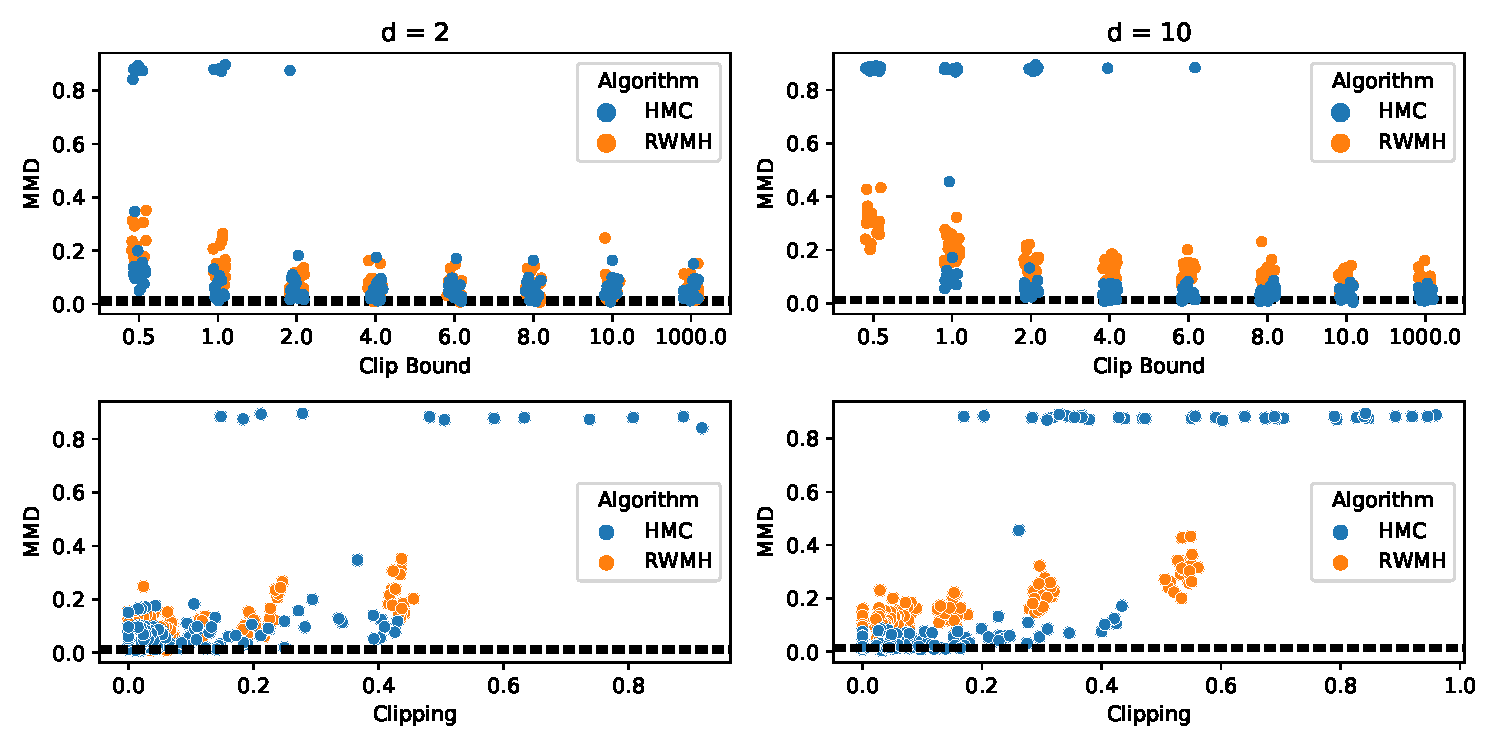
\includegraphics[width=\textwidth]{figures/clipping.pdf}
    \caption{
        The effect of log likelihood ratio clipping on the posterior of the 
        banana model for random walk Metropolis-Hastings and HMC.
        The top row shows posterior MMD as a function of the clip bound, and 
        the bottom row shows MMD as a function of the fraction of log likelihoods 
        that were clipped. The left columns used a 2-dimensional posterior 
        while the right columns had a 10-dimensional posterior. 
        The black lines show the MMDs ten different samples of the true posterior
        compared to the reference sample. All of the lines are close the each 
        other and appear as a single line.
    }
    \label{clip_effect_fig}
\end{figure}
% \section{Accuracy of CLT With Subsampling}

\section{Illustrating HMC}
\section{Banana Distribution}

\begin{figure}
  \centering
  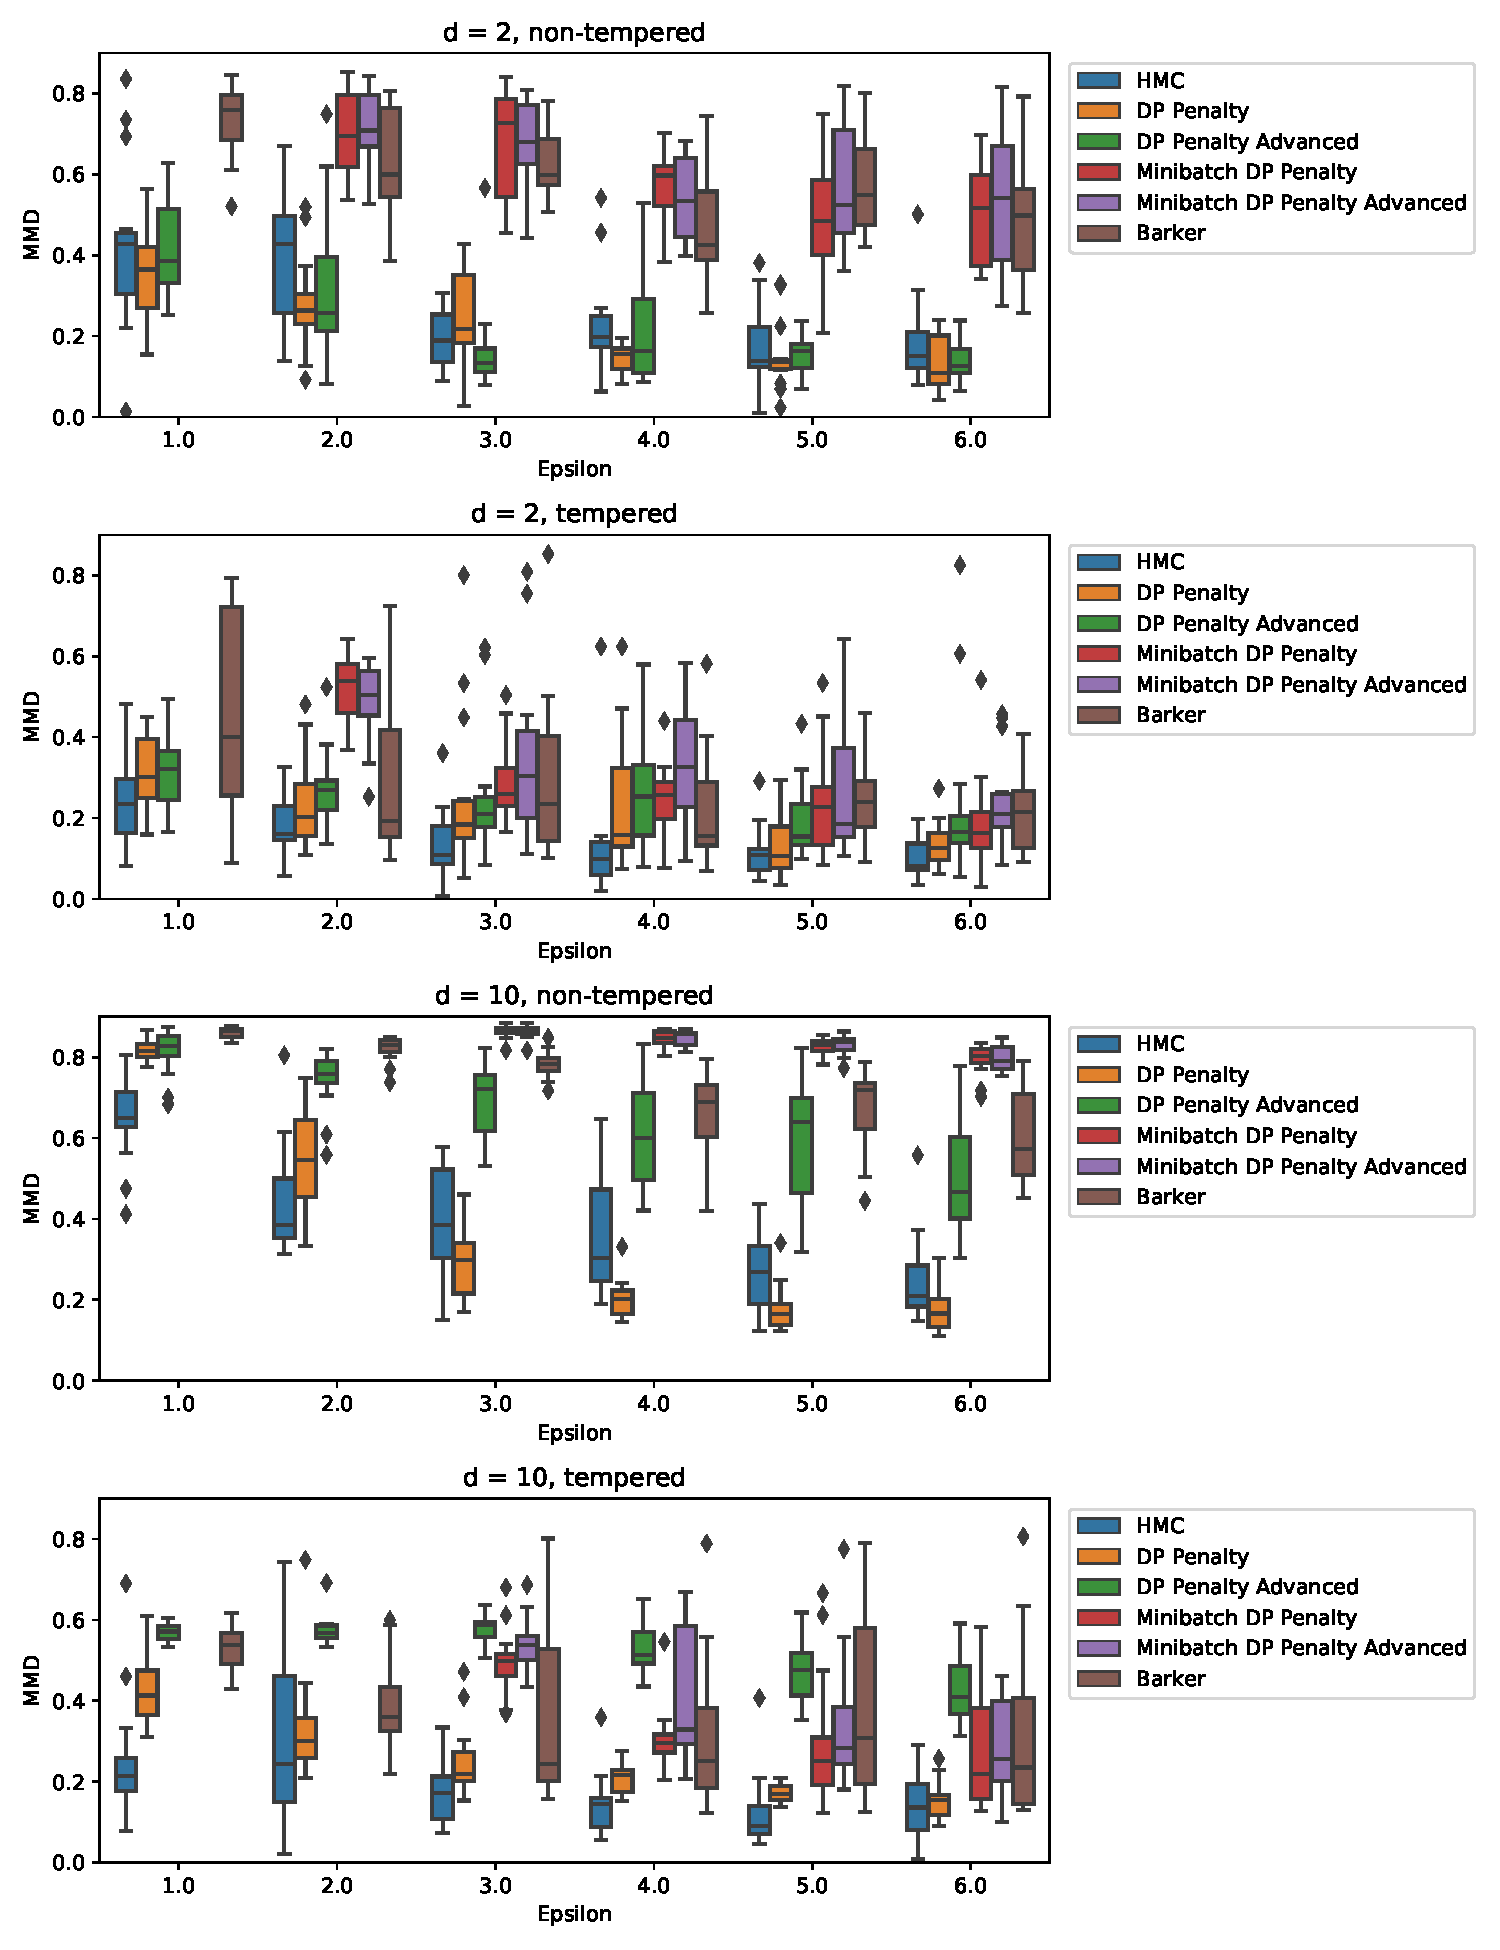
\includegraphics[width=\textwidth]{figures/banana_mmd.pdf}
  \caption{
    MMD as a function of \(\epsilon\) for the different MCMC algorithms,
    with both tempering and a low number of dimensions (2) and a high number
    of dimensions (10).
  }
  \label{banana_mmd_fig}

\end{figure}

\begin{figure}
  \centering
  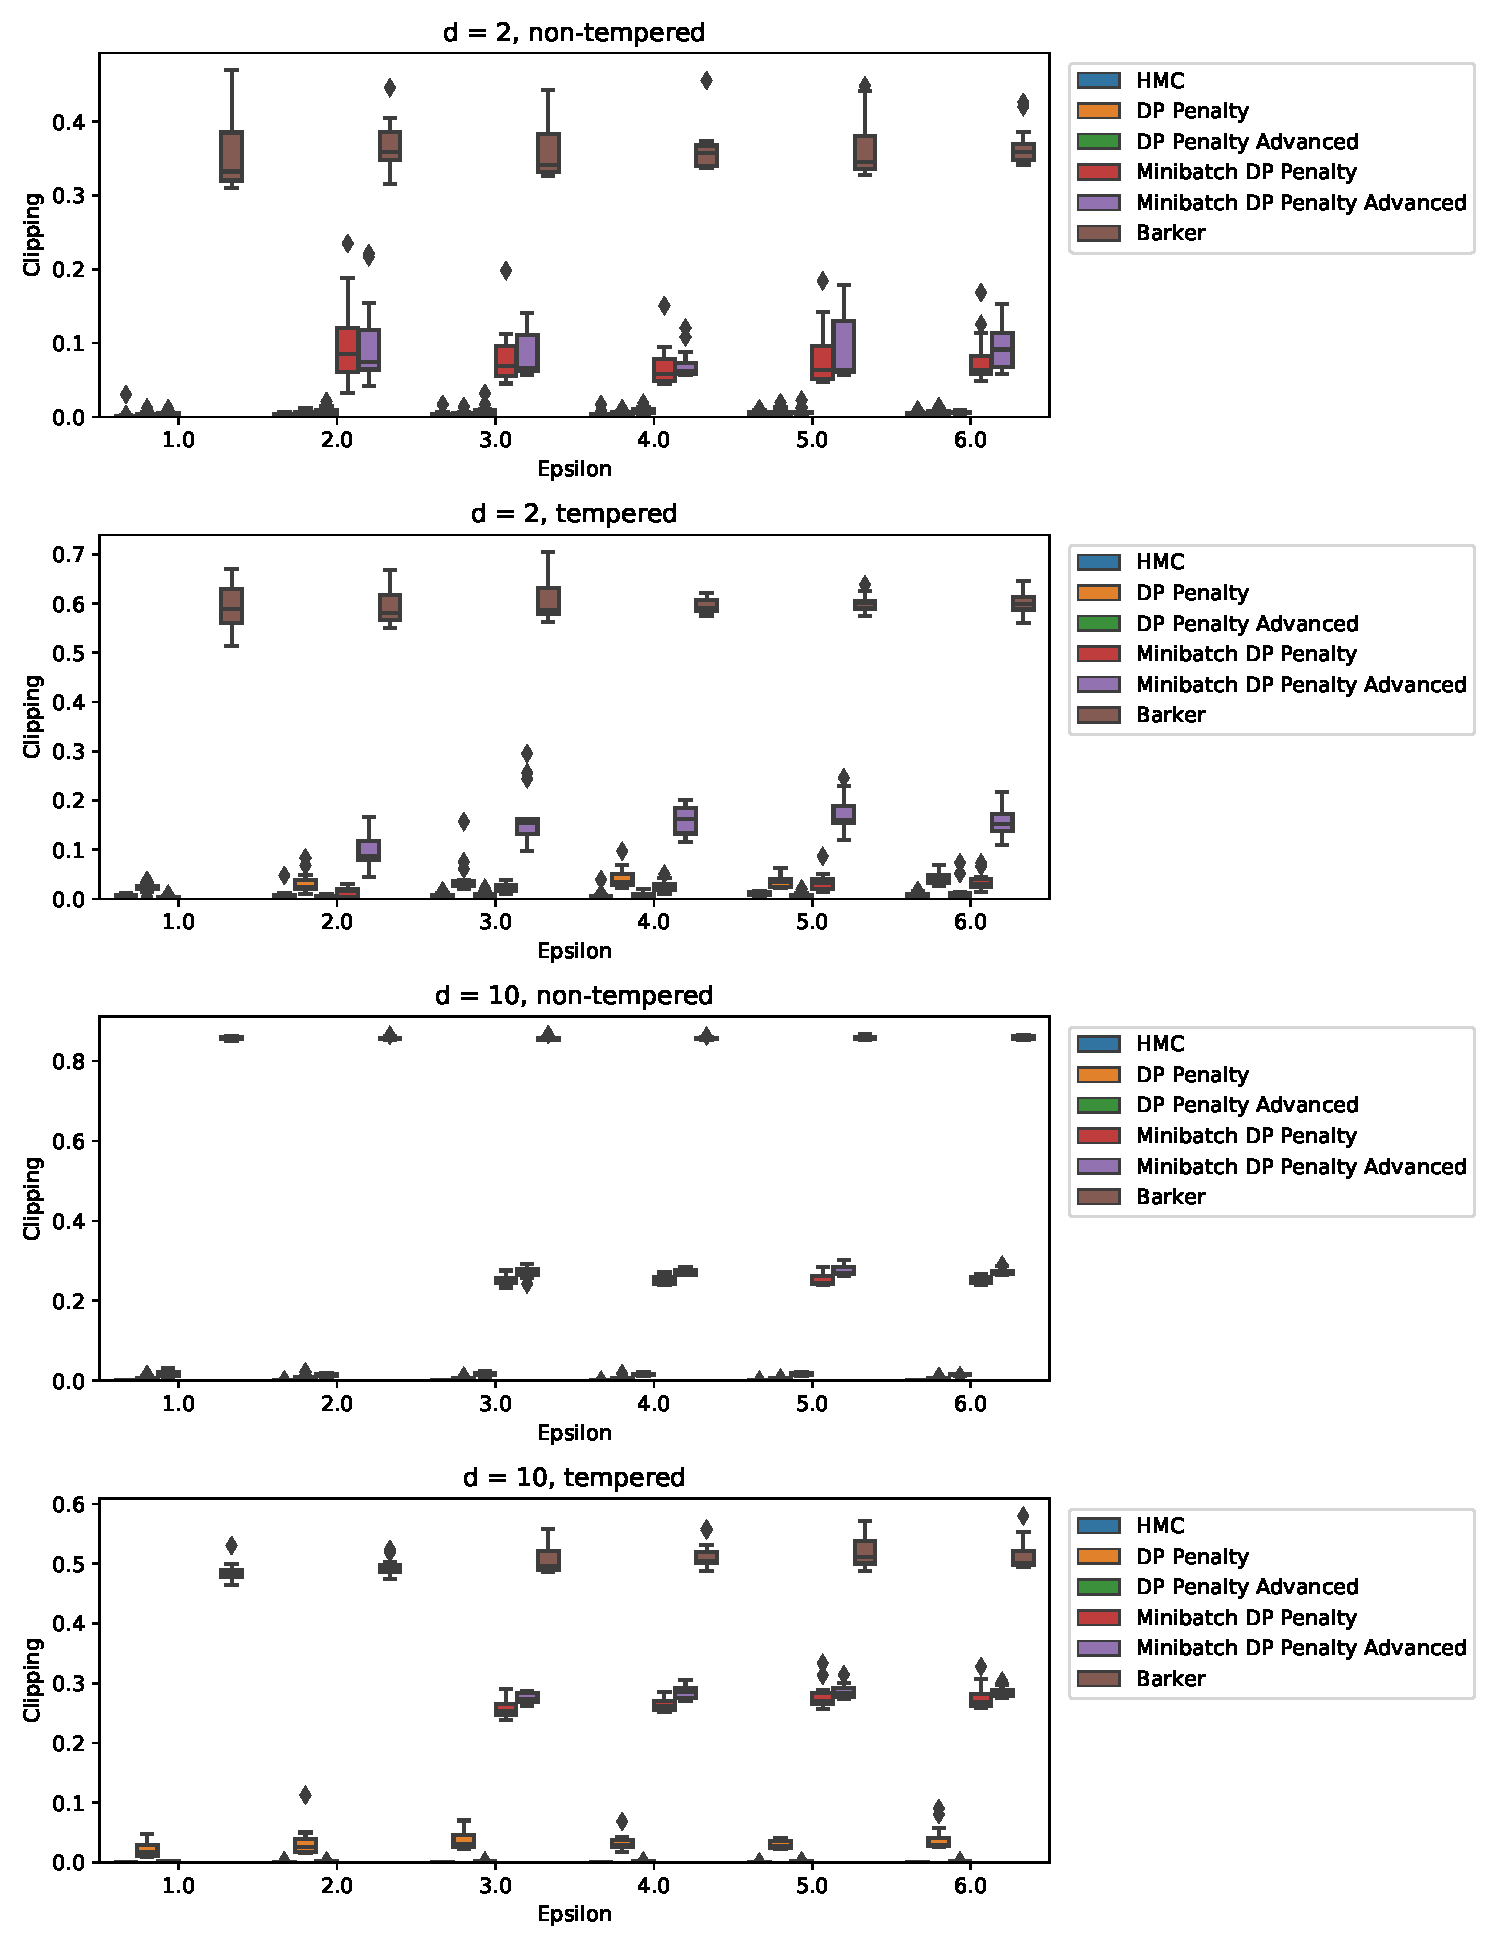
\includegraphics[width=\textwidth]{figures/banana_clipping.pdf}
  % \caption{

  % }
  \label{banana_clipping_fig}
\end{figure}

\begin{figure}
  \centering
  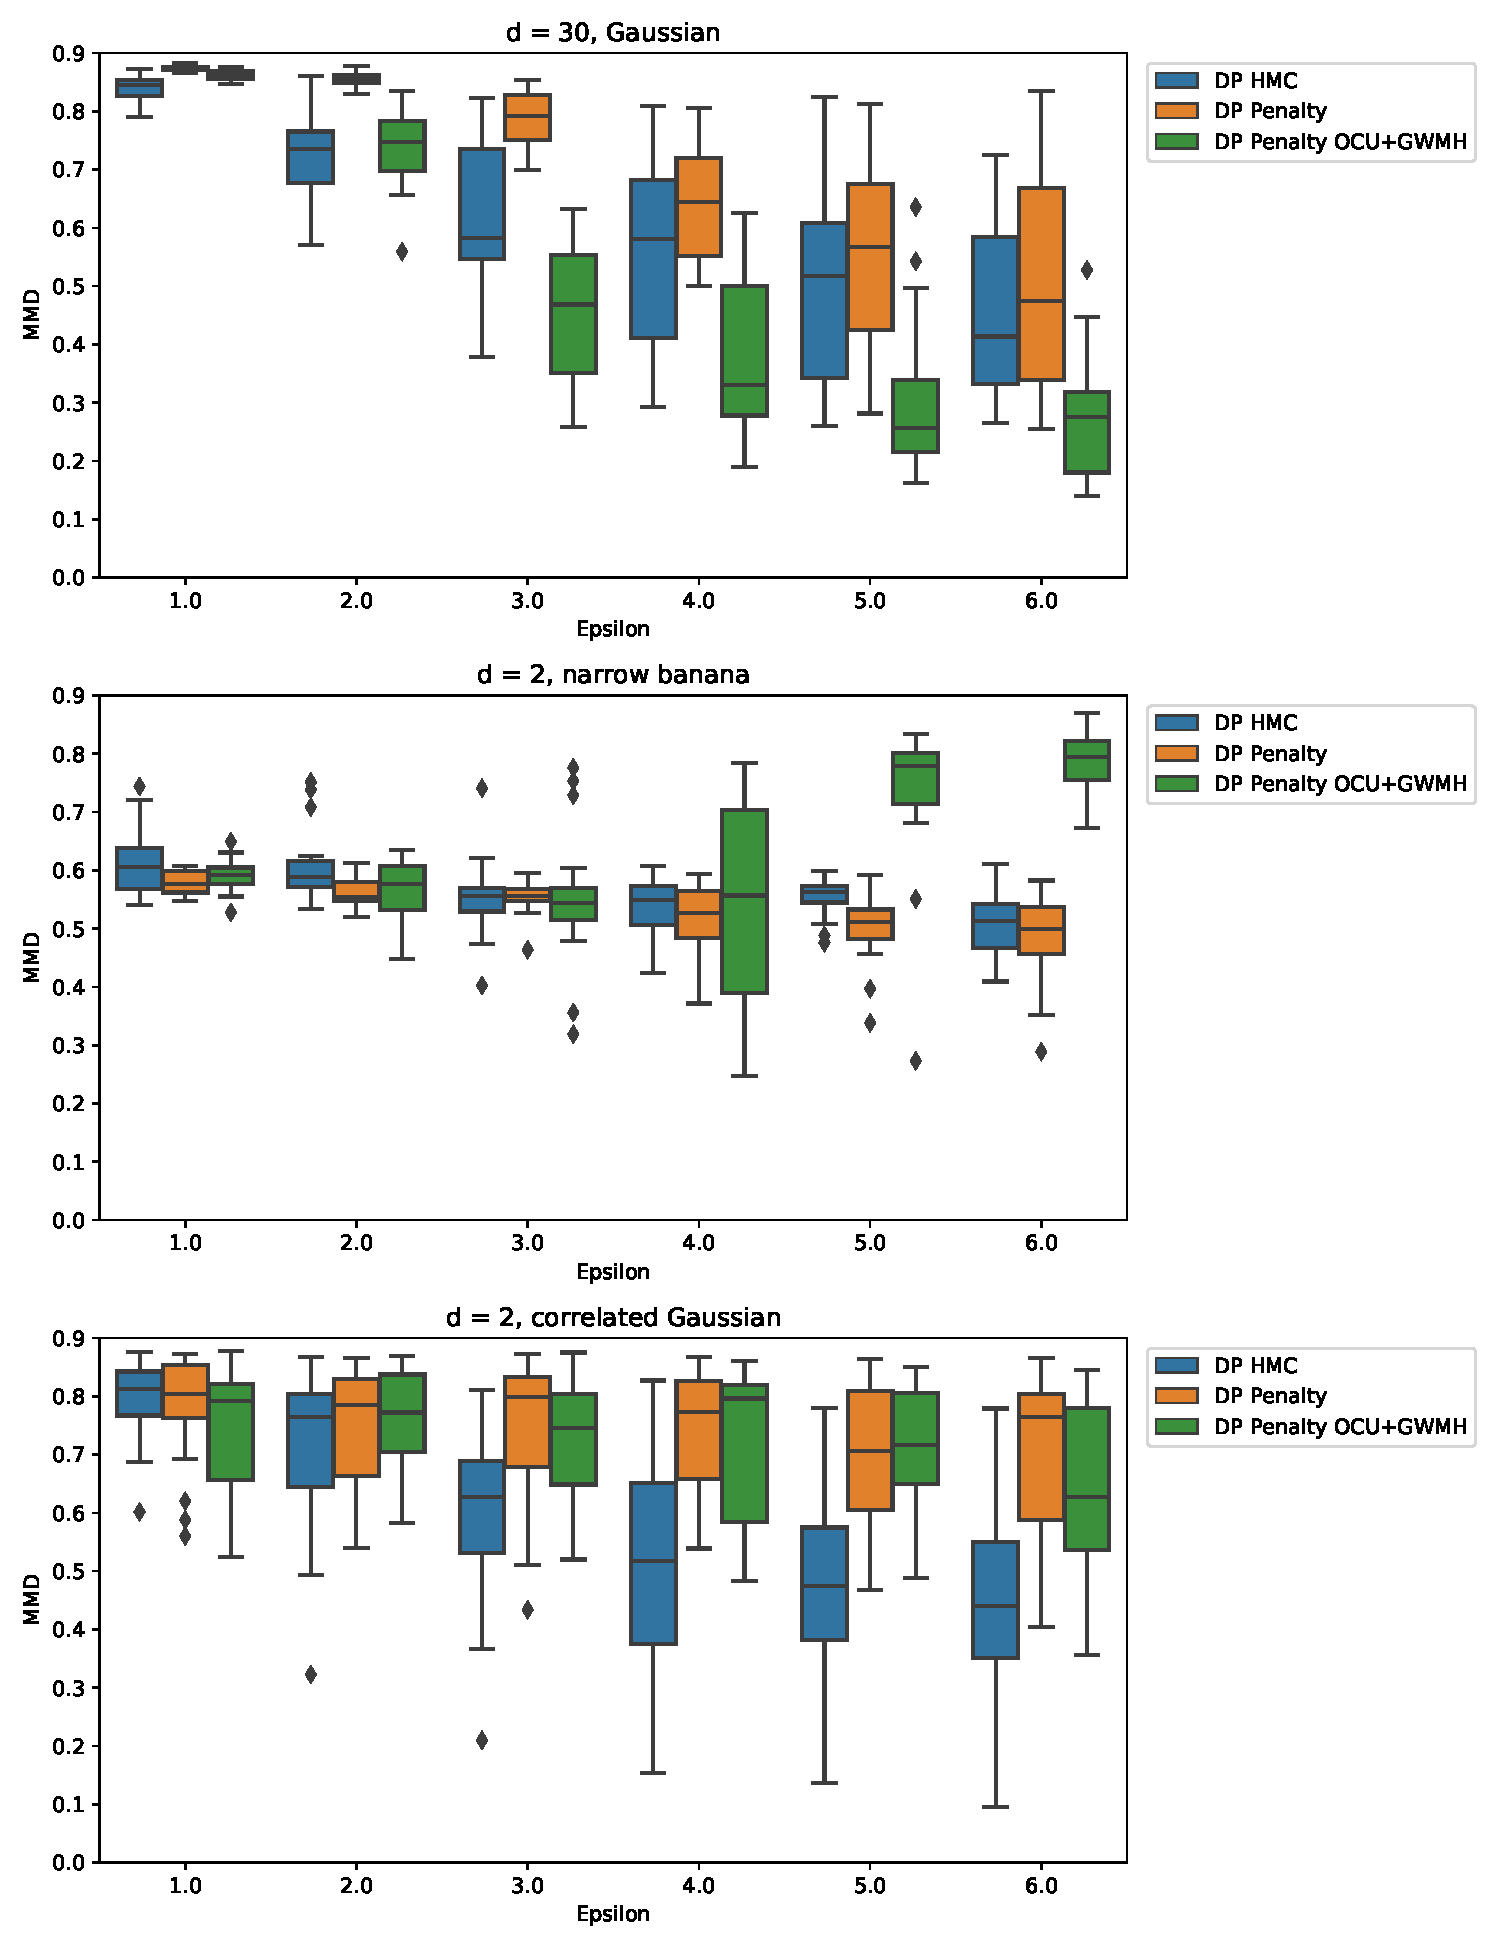
\includegraphics[width=\textwidth]{figures/banana_extra.pdf}
  % \caption{

  % }
  \label{banana_extra_mmd_fig}
\end{figure}

\chapter{Conclusions}
% STEP 5:
% Uncomment the following lines and set your .bib file and desired bibliography style
% to make a bibliography with BibTeX.
% Alternatively you can use the thebibliography environment if you want to add all
% references by hand.

\cleardoublepage %fixes the position of bibliography in bookmarks
\phantomsection

\addcontentsline{toc}{chapter}{\bibname} % This lines adds the bibliography to the ToC
\bibliographystyle{alpha} % numbering alphabetic order
\bibliography{../references.bib}

% \begin{appendices}
% \myappendixtitle
%
% \chapter{Code example\label{appendix:code}}
% Program code can be added as appendix:
% \begin{verbatim}
% #!/bin/bash          
% text="Hello World!"
% echo $text
% \end{verbatim}
%
% \end{appendices}

\end{document}
